\documentclass[11pt,a4paper]{article}
\usepackage{graphicx}
\usepackage{amsmath}
\usepackage[breaklinks=true]{hyperref}
\usepackage{chemarr}
%\usepackage[backend=bibtex,style=numeric-comp]{biblatex}

%\bibliography{dinamica}

\title{DINAMICA 1.0:\\Automated Dynamical Analysis}
\author{Ilya Potapov}
\date{}

\begin{document}
\maketitle{}

\newpage{}

\tableofcontents

\newpage{}

\section{Introduction}
\label{sec:introduction}

DINAMICA is a tool for automated analysis of the multi-stable dynamics. For this, it
uses the differential equation tools supplied with various stochastic validation
algorithms. Consequently, DINAMICA can be used as a tool for the comparative analysis
between the deterministic and the corresponding stochastic systems.

Simple systems usually do not have very complex dynamics. On the other hand, as the
complexity of the system grows the number of possible dynamical regimes increase,
leading inevitably to the co-existing of some of the regimes. In rigid terms, for the
same parameter set the system demonstrates several possible regimes and, as usual
rule for the deterministic systems, different initial conditions lead to the
different dynamics.

The usual assumption in physics, chemistry and biology is that the whole system
consists of the equal elements of smaller size. Thus, DINAMICA considers the equation
supplied by the user to be divided into sub-systems of smaller size. In principle,
these sub-systems must be of the same dimension and all equal in other respects~(the
latter is not required though). Such a system is called a Symmetrically Coupled
System.

\subsection{Interface}
\label{sec:interface}

DINAMICA has a primitive interface with no graphics carried out by the program
itself. It is easy expandable for using the Gnuplot for visualization of results. The
installation process can be done with or without support of the Gnuplot utility. The
Gnuplot is freely available from the Internet.

DINAMICA also uses the external library (Gnu Scientific Library, GSL) to perform some
basic calculations like integration of the system of differential equations,
performing statistics etc. The library can be easily found and downloaded from the
Web and subsequently installed.

These two are the main dependencies of DINAMICA which require the user to have them
pre-installed. Although the Gnuplot is optional, the GSL is mandatory to have
installed on the user's computer.

DINAMICA has been successfully tested on Unix-like OS: Linux, Mac OS X etc. No
testing was performed in the Windows environment, though the Windows use of the
program is NOT prohibited. Any tests for implementation of the software on the new
platforms are much appreciated and all needed help will be provided by the original
author.

The most updated information regarding the interface as well as the installation and
prerequisites instructions can be found in the \texttt{README} file of DINAMICA
package.

\subsection{Disclaimer}
\label{sec:disclaimer}

DINAMICA is distributed as is. The author has no responsibility for the performance of
the software nor for any possible harm or damage the software might cause to the
platform it is run upon. All the details of the disclaimer are explained and further
clarified in the Gnu General Public License.

DINAMICA is free software: you can redistribute it and/or modify it under the terms
of the GNU General Public License as published by the Free Software Foundation,
either version 3 of the License, or (at your option) any later version.

DINAMICA is distributed in the hope that it will be useful, but WITHOUT ANY WARRANTY;
without even the implied warranty of MERCHANTABILITY or FITNESS FOR A PARTICULAR
PURPOSE. See the GNU General Public License for more details.

The License can be found at \texttt{http://www.gnu.org/licenses}\, or in
\texttt{COPYING} file of the package. All the source files of DINAMICA have the
Disclaimer in the beginning along with the copyright information and contact details
of the original author(s).

\subsection{Where To Get}
\label{sec:where-get}

DINAMICA is a part of the free-software community. The description and all source
files needed for the end-user utilization and the development are located in the main
software forge of the Free Software Foundation --- Savannah
(\texttt{http://savannah.gnu.org}). All the latest updates of the program get
uploaded to the Savannah pages dedicated to DINAMICA:

\begin{verbatim}
http://savannah.nongnu.org/projects/din
\end{verbatim}
No special registration is needed, the software is available right there. Various
information about the package and the course of its development can be found on those
pages. For example, the download area contains all public releases of the software:

\begin{verbatim}
http://download.savannah.gnu.org/releases/din/
\end{verbatim}
There is also possibility to become a member of the developers' team if someone is
interested in introducing the new features to DINAMICA. All such efforts are
appreciated. In this regard, the package file \texttt{TODO} is a good opportunity to
see all the new features and capabilities waiting to be realized.

All the changes and updates are recorded in the \texttt{ChangeLog} and
\texttt{NEWS} file of the package. \texttt{ChangeLog} files are also organized by
year, i.e. all updates introduced in 2012 are in \texttt{ChangeLog2012}. The most
recent updates are in \texttt{ChangeLog}.

\subsection{Acknowledgements}
\label{sec:acknowledgements}

The author is thankful to all his teachers in the area of dynamical systems and
stochastic processes, whom he met during the fulfillment of the Masters and Doctoral
thesis. Especially, Prof. Evgenii Volkov (Lebedev Physical Institute, Moscow) and
Andre Ribeiro, PhD (Tampere University of Technology).

The special thanks go to N.Devillard, who has developed the interface for using the
Gnuplot utility from within a C-program \newline (see
\texttt{http://ndevilla.free.fr/gnuplot/}). DINAMICA uses this interface.


\subsection{Installation}
\label{sec:installation}

\textbf{NOTE}: the most recent instructions for the installation process and all
dependent procedures are located in the package \texttt{README} file.

DINAMICA uses AutoConf and AutoMake systems for configuration. The general
information on how to configure the package administrated by these two systems is
located in the \texttt{INSTALL} file of the package.

\subsubsection{Prerequisites}
\label{sec:prerequisites}

\begin{enumerate}
\item Unix/Linux OS.
\item gcc compatible C compiler, needed for Dinamica functioning (not only
  compilation).
\item GNU Scientific Library (GSL) installed.
\item Gnuplot plotting utility installed (optional, but advisable).
\end{enumerate}

\subsubsection{Main Steps of Installation Process}
\label{sec:quick-installation}

\begin{enumerate}
\item Download the archive (usually .zip or .tar.gz) and uncompress it.
\item Configure the system by typing \texttt{./configure}. This will check for all
  the requirements and complain if any of those is not found. You may consider
  \texttt{CPPFLAGS} and \texttt{LDFLAGS} variables, as well as \texttt{--prefix}
  option to \texttt{./configure}, before configuring the system (see below).
\item Type "make" to compile the \texttt{libdin.a} and the \texttt{dinamica}
  itself. The two must appear under the \texttt{src/} directory in the root,
  i.e. where you uncompressed the archive. (It is also important to know why we need
  these two files for the software to work.)
\item Type \texttt{make install} to install \texttt{dinamica} executable and
  \texttt{libdin.a} library to the usual destinations (\texttt{/usr/local/bin} and
  \texttt{/usr/local/lib}, respectively). This might require the root password. You
  may uninstall the program later by typing \texttt{make uninstall} to remove those
  two files from the system. After the installation one might want to remove all the
  files extracted from the archive.
\end{enumerate}

\subsubsection{Important to Know Before Configuring the Package}
\label{sec:import-know-before}

DINAMICA processes the input from the user (equations, parameters, variables,
constants etc.) in the form of the file having \texttt{.ode} extension (ode-file, for
short). The result of the processing is the output \texttt{.c} file with C language
definitions and functions for the user system and the binary configuration
\texttt{.bcf} file. This output \texttt{.c} file is then compiled with the DINAMICA
library (\texttt{libdin.*}) generating the final executable \texttt{.din}. This
executable is then invoked to read the \texttt{.bcf} file and, finally, the program
fires up. Schematically this process is shown in Fig.~\ref{fig:1}.

\begin{figure}[h]
  \centering
  \includegraphics[scale=0.6]{working_scheme}
  \caption{The general scheme representing the DINAMICA preparation procedures before
    it starts.}
  \label{fig:1}
\end{figure}

It is important to understand that the compilation and linking of the libraries
take place during the functioning of DINAMICA. Thus, the compiler and the right
path for the required libraries are needed to be properly set when DINAMICA is
first compiled. One should take care of this before the configuration starts.

The way DINAMICA can obtain the full set of the paths is to specify
\texttt{CPPFLAGS}, \texttt{LDFLAGS} and \texttt{--prefix} option, together or one by
one when needed. These three variables are passed to the DINAMICA compilation
command, so they are crucial. The current directory where DINAMICA is invoked is
always checked for the dinamica library (\texttt{libdin.so} or \texttt{libdin.a}).

\paragraph{CPPFLAGS.}
\label{sec:cppflags}

This variable is important for the preprocessor, a program checking the included, so
called header, files. During the configuration process the \texttt{./configure}
script checks for several \texttt{.h} files from the GSL and the standard C libraries
whether they are available. Sometimes it fails to find them in the standard
locations. In this case, the \texttt{CPPFLAGS} is needed. The usage is simple: if one
knows that the GSL headers are located, for example, in \texttt{/usr/local/include/},
e.g. the full path to \texttt{gsl\_odeiv2.h} file is\newline
\texttt{/usr/local/include/gsl/gsl\_odeiv2.h} (similarly for all other gsl
\texttt{*.h} files), then one could type at the shell prompt:

\begin{verbatim}
CPPFLAGS=/usr/local/include ./configure
\end{verbatim}
This sets the environment variable for the \texttt{./configure} script.  Next, in
DINAMICA this variable will be set after the \texttt{-I} flag of the compiler, i.e.
will also be used as a path to the header files to find (since DINAMICA uses the same
set of header files to compile the user-defined \texttt{.c} file). Note, that the
path to the GSL header files is always \texttt{gsl/*.h}, so omit the \texttt{gsl/}
directory when specifying the \texttt{CPPFLAGS} like in the example provided.

\paragraph{LDFLAGS.}
\label{sec:ldflags}

This variable shows the path to the GSL library (and possibly the standard C
libraries). If the gsl library files are located in \texttt{/usr/local/lib} then
combining with \texttt{CPPFLAGS} one could type

\begin{verbatim}
CPPFLAGS=/usr/local/include LDFLAGS=/usr/local/lib ./configure
\end{verbatim}
which should do the trick. Additionally, DINAMICA will compile the output \texttt{.c}
file against the \texttt{libdin.so/libdin.a} using this variable or the one specified
by \texttt{--prefix} (see below) to find the \texttt{libdin.so/libdin.a}
library. This value will go to the \texttt{-L} flag of the compiler, which specifies
the path to the libraries to be used in the compilation.

\paragraph{- - prefix.}
\label{sec:-prefix}

\texttt{./configure} script accepts the \texttt{--prefix} option, which specifies the
installation directory for \texttt{make install} command. Namely,

\begin{verbatim}
./configure --prefix=/usr/local
\end{verbatim}
would install all the files produced by the package to the corresponding
subdirectories of \texttt{/usr/local}. For example, binary files, i.e
\texttt{dinamica}, would go into \texttt{/usr/local/bin} and libraries,
i.e. libdin.a, --- into \texttt{/usr/local/lib}. This variable is set after the
\texttt{-L} flag to the compiler in DINAMICA.

\subsection{Running DINAMICA}
\label{sec:running-dinamica}

The most simple invocation of DINAMICA is to type at the command line:
\begin{verbatim}
dinamica <your_ode_file>.ode
\end{verbatim}
This will fire up the program, if the configuration and installation processes went
well. \texttt{<your\_ode\_file>.ode} is the \texttt{.ode} file containing the system
to be analyzed. This file should be prepared by the user.

The program starts by showing some information about the system it has read from the
\texttt{.ode} file, a little report on the compilation of the transformed \texttt{.c}
file against the DINAMICA library (\texttt{libdin.so}) and some miscellaneous
information. A typical output looks like:
\begin{verbatim}
<here is your prompt>$ dinamica bruss2.ode 
Starting to check system's specification:
Rebuilding the function:
f(x,y)=a-(b+1)*x+y*x^2
Rebuilding the function:
g(x,y)=b*x-y*x^2
u1' = f(u1,v1)
v1' = g(u1,v1)+dv*(v2-v1)
u2' = f(u2,v2)
v2' = g(u2,v2)+dv*(v1-v2)
Starting transfer to `bruss2.c'...
Done.
Active parameters: `b', `a', `dv', 
Writing `bruss2.bcf'...Done.
Preparing for `bruss2.c' compiling...
Compiling with: `gcc -Wall bruss2.c
-I/opt/local/include -L/opt/local/lib -L./
-o bruss2.din -ldin -lgsl -lgslcblas -lm '
Starting bruss2.din...
./bruss2.din bruss2.bcf 


DINAMICA Ver. 1.0 (<dl.sv.nongnu.org/releases/din/>)
Copyright 2008, 2009, 2010, 2011, 2012, 2013, 2014 Elias Potapov

Copyright 1996, 1997, 1998, 1999, 2000, 2001, 2002, 2003, 2004, 
2005, 2006, 2007, 2008, 2009, 2010, 2011 The GSL Team

This software uses the gnuplot_i library written by N.Devillard
(see <http://ndevilla.free.fr/gnuplot/>).

This program comes with ABSOLUTELY NO WARRANTY;
for details type `warranty' or simply `w'
This is free software, and you are welcome to redistribute it
under certain conditions; see GNU General Public License for details.

Report bugs to <elias.potapov@gmail.com>


Reading `bruss2.bcf'...Done.

>
\end{verbatim}
Then the DINAMICA's own command line (\texttt{>}) is shown up.

DINAMICA is organized in menus, which have a certain hierarchy that does not go
deeper than 2-3 levels starting from the main menu and ending at submenus. The
ubiquitous commands are \texttt{ls} and \texttt{sh}/\texttt{show}~(not
everywhere). The former shows the list of possible menu items and the command
shortcuts to access them, while the latter shows the information corresponding to a
certain type of menu.

The menu items are shown such that the shortest command abbreviation for invocation
of this particular menu is surrounded with parentheses. For example, menu item
\texttt{(N)umerics} can be accessed by typing \texttt{n} at the DINAMICA prompt. The
main menu look like:
\begin{verbatim}
>ls
MAIN menu:
(R)un*
(R)un (t)ransient*
(R)un (i)nitial*
(C)alculate*/
(F)ile/
(N)umerics/
(P)arameters*
(V)ariables*
P(e)riodics/
(G)raphics/
(I)nitials*
(T)rajectory/
C(o)ntinue/
R(a)ndom/
(Er)rors/
(S)ingularity/
(L)yapunov/
(R)un (l)inear*
\end{verbatim}
Some more examples to clarify the concept, to access \texttt{File} menu one should
type in \texttt{f} at the prompt, to run system for the transient amount of time type
in \texttt{rt} etc.

The main menu also has the sign showing the type of the submenu. A slash \texttt{'/'}
at the end of menu item tells a user that this is a regular menu, while an asterisk
\texttt{'*'} tells about a command to be invoked.

Every command released at the prompt needs an 'Enter' key hit at the end to be
accepted by the DINAMICA interpreter. One can use several commands in a row to access
more items in the submenus. For example, to show the numerics information of the
systems one could type in \texttt{n}, 'Enter', \texttt{sh} which will first bring the
user to the \texttt{Numerics} submenu and then in that particular submenu the
\texttt{show} command is invoked. Alternatively, the same result in a rather faster
way can be achieved by typing \texttt{n sh} at the prompt. This is quite
self-explanatory.
\begin{verbatim}
>n sh
* Dimension: 4
* Number of systems: 2
* Number of parameters: 3
* Number of user functions: 2
* Number of auxillary entities: 0
***************************
Total time: 50
Transient time: 50
Step: 0.02
Writing step: 1
Sampling frequency: 1.00
Method: rkf45
Langevin flag: false
\end{verbatim}



\section{Input Files}
\label{sec:input-files}

\subsection{ODE Files}
\label{sec:ode-files}

This type of files is the main source for DINAMICA. Certainly, men must tell software
what to do, that is why \texttt{.ode} files preparation mostly lies upon the user's
shoulders. First, we will present some general examples of using \texttt{.ode} files,
which will provide one with a good basis to start his/her own research almost
immediately once the examples are understood. Next, we will try to draw the detailed
explanation on how the \texttt{.ode} files are constructed and what is the main
syntax and usual pitfalls one might encounter during the declaration of his/her own
system.

\subsubsection{Two Start-off Examples}
\label{sec:two-start-examples}

Let's start from the simple example we used before for invocation of
DINAMICA:
\begin{verbatim}
# bruss2.ode
# two Brusselator coupled by the diffusion equations

%system 2

du1/dt=f(u1,v1)
dv1/dt=g(u1,v1)+dv*(v2-v1)
du2/dt=f(u2,v2)
dv2/dt=g(u2,v2)+dv*(v1-v2)

f(x,y)=a-(b+1)*x+y*x^2
g(x,y)=b*x-y*x^2

jac u1=-(b+1)+2*v1*u1-du,u1^2,du,0
jac v1=b-2*v1*u1,-u1^2-dv,0,dv
jac u2=-(b+1)+2*v2*u2+du,u1^2,-du,0
jac v2=b-2*v2*u2,-u1^2-dv,0,dv

par b=2.5,a=1,dv=.57
init u1=10,u2=1,v1=1.5,v2=15
@ total = 50,yax=v1,yax2=v2
done
\end{verbatim}
This file specifies the systems of two diffusively coupled Brusselators. The system
of Ordinary Differential Equations (ODE's) is written down in a self-explanatory
way. The variables of the system are \texttt{u1}, \texttt{v1}, \texttt{u2} and
\texttt{v2}. Everything that is not a variable in the ODE's is either parameter or
function/auxillary entity. Thus, \texttt{dv} is a parameter, while \texttt{f} and
\texttt{g} are the functions whose definition follows the ODE specification. The
function declaration introduce new parameters: \texttt{a} and \texttt{b}. The
function arguments list is within the parentheses, hence \texttt{(x,y)} denotes two
arguments to the functions.

There is a possibility to include Jacobian into the system declaration. This is used
by several solvers. However, it is not necessary since DINAMICA has a capability of
calculating the Jacobian numerically. That is done automatically, when the program
cannot find the user-supplied Jacobian. The Jacobian is included through \texttt{jac}
statement followed by a variable name whose differential equation is going to be
subject for differentiation. All different derivatives are separated by commas
\texttt{','}\,. Thus, the Jacobian matrix is formed.

\texttt{par} statement specifies the initial values of the parameters of the
system. If some of the parameters are omitted here, their values equal to zero by
default.

\texttt{init} statement does the same job as \texttt{par}, but for the initial values
of the variables. Again, omitted variable values default to zero.

\texttt{@} sign denotes the line with internal parameters for DINAMICA. In the above
example, \texttt{total} means the total time of integration, \texttt{yax} denotes the
variable to be plotted on the Y-axis, \texttt{yax2} denotes the second variable to be
plotted along with the first one on the Y-axis.

\texttt{done} statement is not necessary, but shows the hereditary connection of
DINAMICA to the Bard Ermentrout's XPPAUT software. Actually, the ODE syntax is mainly
like in XPPAUT\newline (see \texttt{http://www.math.pitt.edu/$\sim$bard/xpp/xpp.html}).

As you might have noted the \texttt{\#} sign starts the comments. The very important
DINAMICA directive is \texttt{\%system} which defines number of physical sub-systems
that the whole system has. In the example above, this number is 2, meaning that there
are 2 Brusselators coupled with each other.

This example must provide a start-off principles of defining the ODE systems through
the \texttt{.ode} file.

The next example include the definition of the discrete stochastic system whose
dynamics is going to be compared against the deterministic system of ODE's.
\begin{verbatim}
# Toggle Switch example
# two mutually inhibiting proteins x and y

x'=alpha/(1+y^n)-d*x
y'=alpha/(1+x^n)-d*y

init x=10,y=0
par alpha=1,n=2,d=0.1

g:alpha/(1+x^n);+y
g:alpha/(1+y^n);+x
g:d*x;-x
g:d*y;-y

@method=complex,method2=rkf45,sf=1,total=10000
done
\end{verbatim}
This system has tow ODE's describing the dynamics of two protein species in a Genetic
Toggle Switch. This systems is characterized with the two stable states and
possibility to switch between them. Here you can find another type of variables/ODE
definition --- through \texttt{x'} notation. This totally equals the \texttt{dx/dt}
notation.

The main difference as compared to the first example in this section is the
\texttt{'g:'}s statements closer to the end of the file. These statements define the
Gillespie procedure for solving systems possessing the discrete and stochastic
dynamics. The syntax goes as follows: \texttt{g} is a keyword, everything between
\texttt{':'} and the following \texttt{';'} is known as the propensity of the
chemical reaction and, finally, everything after \texttt{';'} is the update vector,
i.e. the vector (whose elements are separated by commas \texttt{','}) containing the
information on how the numbers of the species involved in the reaction change after
the reaction takes place. In our example, first reaction produces (\texttt{+y}) one
molecule \texttt{y}, while the third one removes (\texttt{-x}) one \texttt{x}
molecule from the reaction space.

Under the section of internal parameters (after \texttt{@}) you can find
\texttt{method=complex} directive which tells DINAMICA to use both stochastic
discrete and normal ODE integration methods altogether and compare the
results. Additionally, \texttt{sf=1} statement tells DINAMICA to use \texttt{sampling
  frequency} for the stochastic simulation equal to 1 (depending on the units used in
the system, it could be seconds, years or ages).

Finally, \texttt{done} finishes the input.

\subsubsection{The Syntax in Details}
\label{sec:syntax-details}

The \texttt{ode} files are the main source for DINAMICA running. The program cannot
start without an appropriate ode file supplied to it. In this section we discuss the
syntax of the ode files in some greater detail. The general rule for ode file syntax
is the every new statement line is separated from others by a \texttt{newline}
symbol.

\paragraph{Comments.}
\label{sec:comments}

Comments in the ode files are marked by \verb'#' sign and everything that follows the
sign until the end of line is ignored by the DINAMICA parser.

\paragraph{Differential equations.}
\label{sec:diff-equat}

The Ordinary Differential Equations~(ODE) determine the list of all variables of the
system as well as the law governing its dynamics. The main syntax for defining ODE's is:
\begin{verbatim}
  dx/dt = ...
  y' = ...
\end{verbatim}

Thus, $x$ and $y$ are declared as variables and the corresponding Right Hand
Sides~(RHS) of the ODE's are determined.

The RHS's are transferred as they are to the corresponding \texttt{.c} file for
further compilation~(see Fig.~\ref{fig:1}). So the operator precedence is determined
exactly the same way it is determined for C-language mathematical expressions. The
C-language principles can be found elsewhere, e.g.~\cite{Cproglang}.

For example, the following system
\begin{verbatim}
dx/dt = 1 + x^2 - y*x
y' = (x+1)*y - y^2*x
\end{verbatim}
will be converted to the corresponding C-function:
\begin{verbatim}
f[0] = 1 + pow(x[0],2) - x[1]*x[0];
f[1] = (x[0]+1)*x[1] - pow(x[1],2)*x[0];
\end{verbatim}
where \verb-f- is an array of the RHS functions, while \verb-x- is an array of
variables in standard C language notation and indexing, starting from 0 for the 1st
equation, 1 for the 2nd and so on. Note also that the \verb-pow- function from the
\texttt{math} C library is used for the power sign \verb-^-. The math library is
included into DINAMICA automatically.

Importantly, DINAMICA first checks the derivatives and extracts the variable
names. Then the actual transferring of the RHS equations starts. All unknown
symbols at this moment are set to be the parameters that can be freely varied from
within the program.

\paragraph{Physical systems.}
\label{sec:defin-phys-syst}

DINAMICA deals only with symmetrical dynamical systems or, at least, those having the
same number of variables. Here, we call a sub-system, defined by a subset of variables
of the whole system, a physical system. For example, there can be two oscillators
coupled to each other. Importantly, these sub-systems are mathematically inside a
single system, however, physically they connote different systems.

Number of physical systems is defined by the \verb-%system- directive that cab appear
anywhere in the text. For example,
\begin{verbatim}
%system 2
\end{verbatim}
defines 2 physical sub-systems.

There is no way to define physical sub-systems in the iteration style. This should be
fixed in the future releases. In contrast, DINAMICA given $N$ sub-systems divides the
whole systems into $N$ equal parts starting from the first variable and finishing by
the last. If one has defined 6 variables $x_1$, $x_2$, $x_3$, $x_4$, $x_5$, and
$x_6$ and $N=2$, then variables $x_1$, $x_2$, and $x_3$ denote sub-system 1, whereas
$x_4$, $x_5$, and $x_6$ belong to the sub-system 2. Similarly, the same system can be
divided into $N=3$ sub-systems. However, $N=4$ will not work and DINAMICA will report
the error in this case, since the sub-systems must contain the same number of
variables.

\paragraph{Parameters.}
\label{sec:parameters}

Parameter values are set through \verb-par- statements:
\begin{verbatim}
par a=1,b=5
\end{verbatim}
The above sets value for the parameter $a$ to 1 and that of $b$ to 5.

All undeclared alpha-numeric entities in the ODE declarations are set to be
parameters. The only way to assign a parameter value is via the \verb-par-
statement. Thus, any parameter that did not appear under the statement will be
assigned a value of zero.

\paragraph{Initial conditions.}
\label{sec:initial-conditions}

The initial conditions for the deterministic simulations can be set with \verb-init-
statement. The line has to be of the form:
\begin{verbatim}
init x=0,y=0
\end{verbatim}
specifying the initial conditions for $x$ and $y$, respectively. Several \verb-init-
statements can be on different lines.

The initial condition can be a parameter. In this case the variable's initial
condition and parameter receive a link, which is preserved throughout the running
session of DINAMICA. If the user simulate a trajectory from the initial condition the
link tells which parameter value to take for which variable. This has the preference
over other methods of setting the initial conditions, for example, from a file.

\paragraph{Functions.}
\label{sec:functions}

Functions can be defined in the ode file facilitating a simpler and more structured
way of representing the system.
\begin{verbatim}
f(x) = ...
g(x,y) = ...
w(x,y,z) = ...
\end{verbatim}
The above examples set the functions for the subsequent use in ODE equations. The
syntax includes the function name followed by the list of arguments~(in parenthesis),
separated with comma. Consider the following self-explanatory example:
\begin{verbatim}
f(x) = x^2
u' = v*f(u)
v' = u
\end{verbatim}
The expression \verb-f(u)- is expanded to \verb-u^2- at the moment of the transfer
to the C-file. Note, that the argument list can contain similar names as those used
in the ODE specification, i.e. the name space of variables of a function is separate
from that of the system. For instance, the following is the same as previous with
\verb-u = y- and \verb-v = x-:
\begin{verbatim}
f(x) = x^2
y' = x*f(y)
x' = y
\end{verbatim}

\paragraph{Auxillary entities.}
\label{sec:auxillary-entities}

DINAMICA allows for using auxillary entities that are some constant expressions. The
auxillary functions can be used in the equations and other mathematical
expressions. The main purpose of using the auxillary entities is to provide a
capability to track certain mathematical relations during the simulations. However,
this capability is not fully supported yet and general advice is to avoid using
auxiliaries.

The main syntax for the auxillary entity is:
\begin{verbatim}
aux R=x*y/(1+a)
\end{verbatim}
The keyword \verb-aux- signifies the  beginning of the auxillary statement.


\paragraph{Jacobian.}
\label{sec:jacobian}

Some of the numerical methods require calculation of Jacobian matrix. This can be
done numerically~(by default). However, if the user doubts the correct numerical
estimates of the Jacobian and if the RHS derivatives are virtually easy to calculate
analytically, it is possible to supply the Jacobian matrix to DINAMICA.

The general form of the Jacobian matrix is:
$$
\left|
  \begin{matrix}
    \dfrac{\partial f_1}{\partial x_1} & \dfrac{\partial f_1}{\partial x_2} & \ldots &
    \dfrac{\partial f_1}{\partial x_n}\\
    \ldots & \ldots & \ldots & \ldots \\
    \ldots & \ldots & \ldots & \ldots \\
    \ldots & \ldots & \ldots & \ldots \\
    \dfrac{\partial f_n}{\partial x_1} & \dfrac{\partial f_n}{\partial x_2} & \ldots &
    \dfrac{\partial f_n}{\partial x_n}\\
  \end{matrix}
\right|
$$
where $f_i$ is a RHS function of $i$-th variable $x_i$. There are total $n$ number of
ODE's and, obviously, the same number of variables.

The keyword for entering the Jacobian is \verb-jac-. After the keyword the variable
name, whose differential equation derivatives to be considered on the line. Then,
after the variable name, the equal sign '=' goes, followed by the expressions of the
derivatives separated by comma ','. For example,
\begin{verbatim}
jac u = 2*u-1,v*u-1
\end{verbatim}
determines the Jacobian entry for the \verb-u- variable.

IMPORTANT: \verb-jac- statement MUST be put in the ode file after ALL ODE
declarations. Since for the very first entry the system parser must know how many
variables are in the system, in other terms, what is the dimension of the system.

In the considered above example, we do not know what is the number of the variable
\verb-u- and hence cannot determine derivatives over which variables are
presented. All we know is that there is a variable \verb-u- in the system and the
dimension of the system is 2 (two entries separated by the comma).

Here is the full functional example of Jacobian statement use:
\begin{verbatim}
u'=a-(b+1)*u+v*u^2
dv/dt=b*u-v*u^2

jac u = -(b+1)+2*v*u,u^2
jac v = b-2*v*u, -u^2
\end{verbatim}
The entries \verb-jac u- and \verb-jac v- can be put in any order, since the
variable name after \verb-jac- determines the equation.

\paragraph{Noise terms.}
\label{sec:noise-terms}

The so called Ito differential equations can be studied in DINAMICA. For this one has
to specify the noise terms in the RHS functions. The Ito differential equations
(sometimes referred to as Langevin equations) has a specific form of the noise term,
that is, some \texttt{amplitude} times the white noise = standard normal distribution
(with 0 mean and variance of 1) multiplied by square root of the time step, namely:
$$Noise = A\times\sqrt{dt}\times N(0,1)\,,$$
where $A$ is the amplitude, $dt$ is a time step and $N(0,1)$ is the standard normal
distribution. The amplitude can be set in DINAMICA using the keyword \verb-lang-:
\begin{verbatim}
lang u=0.1,v=0.01
\end{verbatim}

The variable name signifies the ODE equation to add the noise term to. The
expressions right to the equal sign can contain normal mathematical operators and
parameters.

In order to simulate the stochastic trajectory defined by Langevin equations one has
to enable the corresponding simulation methods: simple Euler method or Milstein
method~(both are fixed step size algorithms). Additionally, the so called
\texttt{Langevin flag} must be turned on. All these options can be found under the
\texttt{Numerics} menu.

\paragraph{Stochastic discrete algorithm.}
\label{sec:stoch-discr-algor}

DINAMICA allows for using the discrete stochastic algorithm when simulating the
trajectories~\cite{GillAlg}. The algorithm was formulated by D.~Gillespie and is of
great use for the systems with small number of molecules. Generally, the algorithm
requires the so called \texttt{propensity} functions to be defined and the
\texttt{update vector} of the chemical reactions. The propensity is analog of the
chemical reaction rate. The update vector defines which chemicals are consumed and
which are produced as a result of the reaction. DINAMICA has the straightforward
algorithm~(referred to in~\cite{GillAlg} as ``Direct'' method) for simulating the
discrete stochastic trajectory.

For example, a chemical reaction $A+B \xrightarrow{k} C$ will be written in DINAMICA
ode file as:
\begin{verbatim}
gill:k*A*B;-A,-B,+C
\end{verbatim}

The keyword for the Gillespie algorithm instruction is \verb-gill-, or simply
\verb-g-, followed by the colon '\texttt{:}'. Then the propensity is defined as
in the example above \verb-k*A*B-, followed by the semicolon '\texttt{;}'. Finally,
the update vector is specified, showing how many molecules were removed~(\verb'-')
from the reaction space and how many were added~(\verb-+-, the plus sign can be
omitted) for each chemical species involved in the reaction.

NOTE: the variable name space used in this approach is global, that is the same as
for the ODE equations. Thus, to define a variable to use for the discrete method one
needs to define the corresponding ODE. This way DINAMICA becomes an excellent tool
for qualitative and quantitative analysis and comparison of both discrete and
continuous deterministic trajectories. If the ODE system being compared with the
corresponding discrete stochastic system does not contain a variable to be used one
can always write an ``empty'' ODE to declare a variable to the program:
\begin{verbatim}
dx/dt = 0
\end{verbatim}

NOTE also, that DINAMICA does not prepare the propensity functions for the
user. Thus, for example, for the chemical equation $A + A \xrightarrow{c} B$ the
propensity must be equal to $c\times A\times(A-1)/2$ and be set explicitly by the user:
\begin{verbatim}
g:c*A*(A-1)/2;-2A,B
\end{verbatim}

Additionally, the update vector should not contain mathematical expressions, i.e. in
the example above two molecules of A are consumed, which is set by \verb'-2A' and NOT
\verb'-2*A'.

\paragraph{Technical parameters.}
\label{sec:techn-param}

Technical parameters are those you specify when dealing with the numerical
simulations~(time of simulation, step etc.), graphics~(what to plot, type of the
plots) and some other. This list can be extended significantly, since DINAMICA
contains a lot of different technical parameters related to many analysis
procedures. Every new release of the software should extend the list
significantly. Though not all the parameters can be defined from within an ode file,
almost all of them can be set from within the running program.

The technical parameters to DINAMICA are usually presented in a form
\verb-<par>=<val>- after \verb-@- sign beginning a line, where \verb-<par>- is a name
of the parameter and \verb-<val>- is its value. The pairs can be separated by comma
inside a single line. For example,
\begin{verbatim}
@total=100,dt=.2
\end{verbatim}

\textbf{total} defines the total time of integration/simulation for the trajectories.

\textbf{dt} defines the time step for numerical integrators. The adaptive step size
algorithms take this as an initial guess for the step.

\textbf{trans} determines so called transient time, that is a time interval that can be
run without producing any output. This is usually used for getting the final
attractor of the system.

\textbf{method}/\textbf{m} defines the method of integration. The possible options can
be: \verb-eu-~(simple Euler fixed step size procedure), \verb=run-kut4=~(Runge-Kutta
(4,5) fixed step size method), \verb-rkf45-~(embedded Runge-Kutta-Fehlberg (4,5)
adaptive size method), \verb-rk8pd-~(embedded Runge-Kutta Prince-Dormand (8,9)
adaptive step method), \verb-rkck-~(embedded Runge-Kutta Cash-Karp (4,5) adaptive
step method), \verb-bsimp-~(Implicit Bulirsch-Stoer method, requiring Jacobian
calculation), \verb-discrete-~(Stochastic Discrete Algorithm from~\cite{GillAlg}),
\verb-milst-~(Milstein method for stochastic ODE's, langevin flag (see below) must be
turned on), \verb-complex-~(complex method calculating deterministic trajectory and
one or several stochastic ones combining them into a single output).

\textbf{method2} defines the method for the deterministic run if
\verb-method=complex-.

\textbf{ws} defines the writing step to the output trajectory file. For example,
\verb-ws=100- will force the integrator to put every 100-th point into the output
file.

\textbf{sf} is sampling frequency for the stochastic discrete
algorithm~\cite{GillAlg}. Determines how often to write the output. For example,
\verb-sf=5- will force the simulator to produce output every 5 sec/min/hours or any
other time units implicitly assumed in the model under study.

\textbf{lf}/\textbf{lang} is a Langevin flag. If set to non-zero value, tells the
program to augment the ODE equations with the noise terms, whose amplitudes must be
defined in the ode file or inside the program.

\textbf{graph}/\textbf{gf} is a graphics flag. Non-zero value indicates that the user
wants to use the Gnuplot output. If the program was compiled with Gnuplot support
this option is by default true. Usually used to suppress the output.

\textbf{xaxis}/\textbf{xax} is a variable name or index for plotting at the X-axis. O
indicates time (default), 1,2,3 etc indicate 1st, 2nd, 3rd etc variable.

\textbf{yaxis}/\textbf{yax}/\textbf{yaxis1}/\textbf{yax1} is a variable name or index
for plotting at the Y-axis. First variable is taken by default.

\textbf{yaxis2}/\textbf{yax2} is an additional variable to plot at the Y-axis.

\textbf{yaxis3}/\textbf{yax3} is yet another additional variable to plot at the
Y-axis. Three is the maximum number of plotted variables at Y-axis.

\textbf{permeth}/\textbf{pm} is either 1 or 0 determining the way the periods are
calculated from the simulated trajectory. 0 indicates the default method of Poincare
sections, 1 indicates the autocorrelation method. The former produces set of values
for period, whereas the latter produces a single value for a trajectory.

\textbf{pervar}/\textbf{pv} is a variable name or index telling which variable to use
to assess the system's period.

\textbf{cross}/\textbf{c} is a Poincare section level. This value determines the
fraction between the max and min of the trajectory. Namely, the section level is
determined by the formula: Poincare section = $(\max(\mathbf{X}) - \min(\mathbf{X}))/C
+ \min(\mathbf{X})$, where $\mathbf{X}$ is an array of points defining the trajectory
and $C$ is the cross value defined by \verb-cross-.


\paragraph{Finishing input.}
\label{sec:finishing-input}

The keyword \verb-done- is reserved for the final statement in the ode file. This is
\textbf{optional} and kept for the backwards compatibility as well as compatibility
with XPPAUT ode files~\cite{XppautLink}.

\section{Simulation Methods}
\label{sec:simulation-methods}

The simulation methods in DINAMICA can be divided roughly into two big classes:
deterministic and stochastic.

\subsection{Deterministic Methods}
\label{sec:determ-meth}

These methods are primarily obtained from the GNU Scientific
Library~(GSL)~\cite{GSLLink}. The methods are intended for the numerical simulation
of the system of ODE's. Although there are a plenty of methods for the purpose in the
GSL library, we have opted to use several methods. For the very same reason, the
DINAMICA set of algorithms can be easily extended using the GSL.

\paragraph{Euler 2-nd order.}
\label{sec:euler-2-nd}

The simplest fixed step size approach to solve the system of ODE's. The routine for
the procedure is not from the GSL library.

\paragraph{Runge-Kutta 4-th order.}
\label{sec:runge-kutta-4}

Explicit (classical) 4-th order Runge-Kutta algorithm. Own routine.

\paragraph{Runge-Kutta-Fehlberg 4-th order.}
\label{sec:run-kut-feglberg}

Explicit embedded Runge-Kutta-Fehlberg (4,5) method. This method is a good
general-purpose integrator. This is from GSL: \texttt{gsl\_odeiv2\_step\_rkf45} step
function~(see GSL reference available at~\cite{GSLLink}).

\paragraph{Runge-Kutta Prince-Dormand 8-th order.}
\label{sec:runge-kutta-prince}

Explicit embedded Runge-Kutta Prince-Dormand (8, 9) method. From GSL:
\texttt{gsl\_odeiv2\_step\_rk8pd}.

\paragraph{Runge-Kutta Cash-Karp 4-th order.}
\label{sec:runge-kutta-cash}

Explicit embedded Runge-Kutta Cash-Karp (4,5) method. From GSL:
\texttt{gsl\_odeiv2\_step\_rkck} step function.

\paragraph{Implicit Bulirsch-Stoer method.}
\label{sec:impl-bulirsch-stoer}

Implicit Bulirsch-Stoer method of Bader and Deuflhard. The method is generally
suitable for stiff problems. This stepper requires the Jacobian. From GSL:
\texttt{gsl\_odeiv2\_step\_bsimp}.

\subsection{Stochastic Methods}
\label{sec:stochastic-methods}

These methods can be both continuous and discrete in nature.

\paragraph{Discrete.}
\label{sec:discrete}

The discrete stochastic simulation follows the algorithm described by D.~Gillespie
in~\cite{GillAlg}~(``Direct'' method for the Monte-Carlo step).

\paragraph{Continuous.}
\label{sec:continuous}

This option refers to the Ito stochastic differential equations, also known as
Langevin equations. The general form of the equation of this type is:
\begin{equation}
  \label{eq:lang_eq_general_type}
  \frac{dx}{dt} = f(x) + g(x)\times dW\,,
\end{equation}
where $f(x)$ is a normal RHS of an ODE, $g(x)$ is the function determining the
amplitude of the noise and $dW$ is a Wiener process.

For solving this type of a problem one can choose either the Euler procedure or
the special Milstein method for solving Ito differential equations. For both toggling
of the Langevin flag~(see manual on \texttt{Numerics} menu) is required.

\subsection{Complex Method}
\label{sec:complex-method}

Complex method is a special feature of DINAMICA, which allows for simultaneous
simulation of both stochastic and deterministic counterparts of a system, further
facilitating the comparative analysis of them. This method is designed so that it
first simulates the deterministic part of the system and then several times the
stochastic part, be it discrete or continuous.

The complex methods requires specifying the deterministic algorithm. The stochastic
algorithm is chosen automatically based on whether the langevin flag or the discrete
algorithm are set.

\section[Trajectory System]{Dynamical Analysis Methods: \\Trajectory System}
\label{sec:dynam-analys-meth}

For the analysis of the dynamics DINAMICA uses the simulated time series. At the
moment, all methodology described in this section refers only to the deterministic
time series that is obtained from the simulation of a system described in terms of
Ordinary Differential Equations (ODE's). However, the actual core algorithms for the
dynamical analysis do not need a special means for trajectory generation, only the
deterministic property is required.

\begin{quotation}
Note, that the analysis can be applied to any system described in terms of ODE's,
hence, it is irrelevant what is the independent variable of the system is. Throughout
this manual we use term ``time'' as the independent variable when describing the
algorithms, however, it can be a spatial variable, for example, for some specific
systems. Moreover, we assume that the independent variable is increasing from the
beginning to the end of the simulated trajectory as, usually, happens with time
variable. Thus, for example, the point $i$ of the trajectory takes place for the
larger value of time~(or other independent variable) than the point $i-1$.
\end{quotation}

The set of ODE's represents the system under study mathematically. The system,
however, can be further divided into physical sub-systems representing the actual
coupled physical elements. Although indiscernible mathematically such systems as a
whole may produce a significant differences in the dynamics of the physical
sub-systems~(see e.g.~\cite{Ullner2008}).

First, DINAMICA analyzes the dynamics of 1D system: either the whole system, if the
system's physical dimension is equal to 1, or every sub-system~(number of physical
sub-systems is determined in the \texttt{\%system} directive in the \texttt{.ode}
file). Next, the whole system analysis is fulfilled producing the overall dynamics
report.

The analysis is based upon the concept of \textit{slope}. The next section
explains in detail the concept. Then, we present the slope algorithm for 1D
systems~(meaning systems with the only physical dimension) and, finally, the
procedure for ND systems.

\subsection{The Slope Concept}
\label{sec:concept-slope}

Once the deterministic time series is simulated it can be analyzed through the
DINAMICA \texttt{TRAJECTORY}-system (or \texttt{T}-system). The elementary unit the
whole analysis relies upon is \textit{slope}\,. The slope is a part of the calculated
trajectory (or the time series) from the beginning of section, where the trajectory's
points start to decline over time, up to the beginning of section, where the points
start to ascend over time, or vice versa. The concept is illustrated in
Fig.~\ref{fig:2}.

\begin{figure}[h]
  \centering
  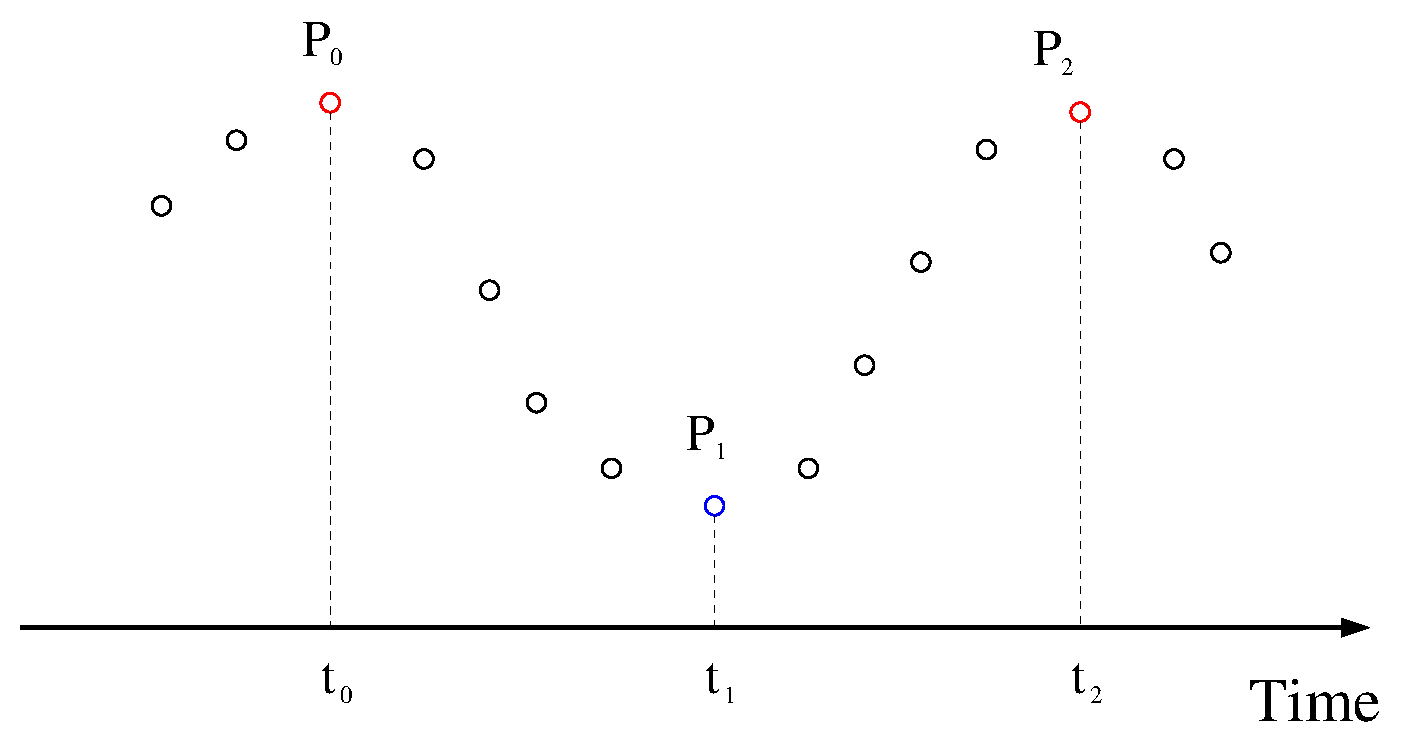
\includegraphics[scale=0.55]{slope}
  \caption{The graphical representation of the slope concept}
  \label{fig:2}
\end{figure}

The set of calculated points belonging to the trajectory has \textit{turning
  points}\,, at which the trajectory changes its direction from pointing upwards to
pointing downwards, or vice versa. Strictly speaking in terms of continuous
trajectory and infinitesimal time step, at those points the corresponding variable's
derivative becomes equal zero.

In Fig.~\ref{fig:2} these points are depicted in red and blue ($P_0$, $P_1$ and
$P_2$) demarcating two slopes: the first contains all the points from point $P_0$ up
to $P_1$ inclusively and the second --- from $P_1$ to $P_2$.

Practically speaking, all kinds of trajectories contain the slopes, since in the most
cases the calculated points have at least small discrepancies in their values caused
by the computer representation of the real numbers. Nevertheless, in those really
rare cases, when two adjacent points have values that are the same (up to the all
representation bits of the numbers), the T-system determines the \textit{plateau},
and the beginning and/or end of the slope is calculated as the point in the center of
plateau (if the plateau contains even number of points the ceiling operation is
taken).

Thus, one can distinguish between \textit{ascending} and \textit{descending}
slopes. In Fig.~\ref{fig:2} the first slope is descending (from $P_0$ to $P_1$),
while the second one (from $P_1$ to $P_2$) is ascending. For the obvious reasons, the
ascending and descending slopes alternate over time. Additionally, the end of each
slope is the beginning of the next one. For this reason, for example, the T-system of
DINAMICA stores only the time that the slope starts at. Using the example depicted in
Fig.~\ref{fig:2}, only $t_0$ and $t_1$ are stored for the two slopes shown.

There are three entities that describe a slope in DINAMICA. The slope
\textit{amplitude} $S^A$ is the difference between the variable values at the beginning and
at the end of the slope. The slope \textit{base} $S^B$ is the lowest point of the
slope. The beginning of the slope in time $S^T$ is the third entity.

Continuing with the example of Fig.~\ref{fig:2}, the slope appearing earlier in time
has amplitude equal to $(P_0-P_1)$, base --- $P_1$ and the start time --- $t_0$,
while the later appearing slope has amplitude equal to $(P_2-P_1)$, base --- $P_1$ and
the start time --- $t_1$. As a result, two adjacent slopes (descending and then
ascending) have the common base.

\subsection{1D Dynamical Analysis}
\label{sec:dynam-regime-detect}

DINAMICA processes the simulated time series of a single variable within the first
physical dimension of the system. All dynamics detection is based on the slope
analysis of the simulated trajectory. The process could be virtually divided into the
\textit{preparation} stage and actual slope algorithm.

The preparation process starts with the calculation of the peaks and troughs of the
simulated trajectory (in Fig.~\ref{fig:2} points $P_0$ and $P_2$ are peaks and point
$P_1$ is a trough). Then, based on the peak and trough information the slopes of the
trajectory are calculated. Next, the slopes are checked to represent real slopes of
the trajectory and not small ``fluctuations'' of it. These small fluctuations appear
in systems with very different timescales, e.g. when there are very slow and very
fast equations in the system. The ``fluctuations'' appear due to this difference of
the time scales and \textit{not} due to any stochastic forces applied to the
system. Perhaps, a suitable integration algorithm accounting for the stiffness of the
system might resolve this problem. In any case, this ``sanity'' checking of the
slopes does not hamper the whole analysis and, hence, is included in the preliminary
preparation stage of the process.

Before moving to the section explaining the slope algorithm we need to take a look at
the dynamical regimes and the definitions used in DINAMICA for the dynamical
processing.

\subsubsection{Dynamical Regimes of 1D Systems}
\label{sec:dynamical-regimes-1d}

1D (here we refer to the physical dimension) systems can in principle have two types
of dynamics: \textit{stationary} and \textit{non-stationary} behavior. The former
refers to so called steady state of a dynamical system, at which the system
eventually ends up at a stationary point. The latter, oppositely, connotes a behavior
that does not rest at any particular point. The non-stationary behavior contains many
sub-classes of behaviors, ranging from pure oscillatory dynamics with distinguished
period and amplitude to chaos with no certainty in the period and
amplitude.

\textbf{NOTE \#1}: the DINAMICA slope algorithm determines the \textit{genuine}
dynamics of a system in a sense of the realized (really appearing) behavior. For
example, there is no way in the slope algorithm to distinguish between oscillations
induced by the harmonic oscillator and the limit cycle oscillations (the first one is
the linear system possessing the ``center'' fixed point with pure imaginary Lyapunov
numbers, while the second is the non-linear system containing the Hopf bifurcation).

\textbf{NOTE \#2}: DINAMICA is capable of determining the chaotic behavior~--- a
dynamical regime in which the deterministic laws of motion produce unpredictable
behavior. But this capability of the program goes beyond the slope algorithm, which
most likely would produce the ``unknown'' or period-$n$ oscillatory regime (see
below), where $n$ is very large, in the case of chaos.

Thus, the non-stationary dynamical behavior is either oscillations with some
predictable periodicity or chaos. The oscillatory regime can be characterized with
its amplitude and period. While the amplitude value is not qualitatively useful, the
period might be composed of several sub-periods, denoting, if they are present, the
additional frequency of oscillations. This takes place, for instance, in case of the
torus attractor.

Here, we define \textit{period}-$n$ oscillations referring to the oscillatory
trajectory with every oscillation being of the same amplitude and the same level as
those of the $n$-th oscillation \textit{prior} or \textit{next} to the given one. For
example, Fig.~\ref{fig:3} shows two sinusoidal oscillation trends. The first one is
described by the expression $\sin(x)$ and the second one --- by
$\sin(x)+\sin(x/2)$. The former has one frequency of oscillations and the latter one
has a period composed of two sub-periods. The $\sin(x)$ oscillatory regime is
period-1 oscillations, the $\sin(x)+\sin(x/2)$ oscillatory regime is period-2
oscillations.

\begin{figure}
  \centering
  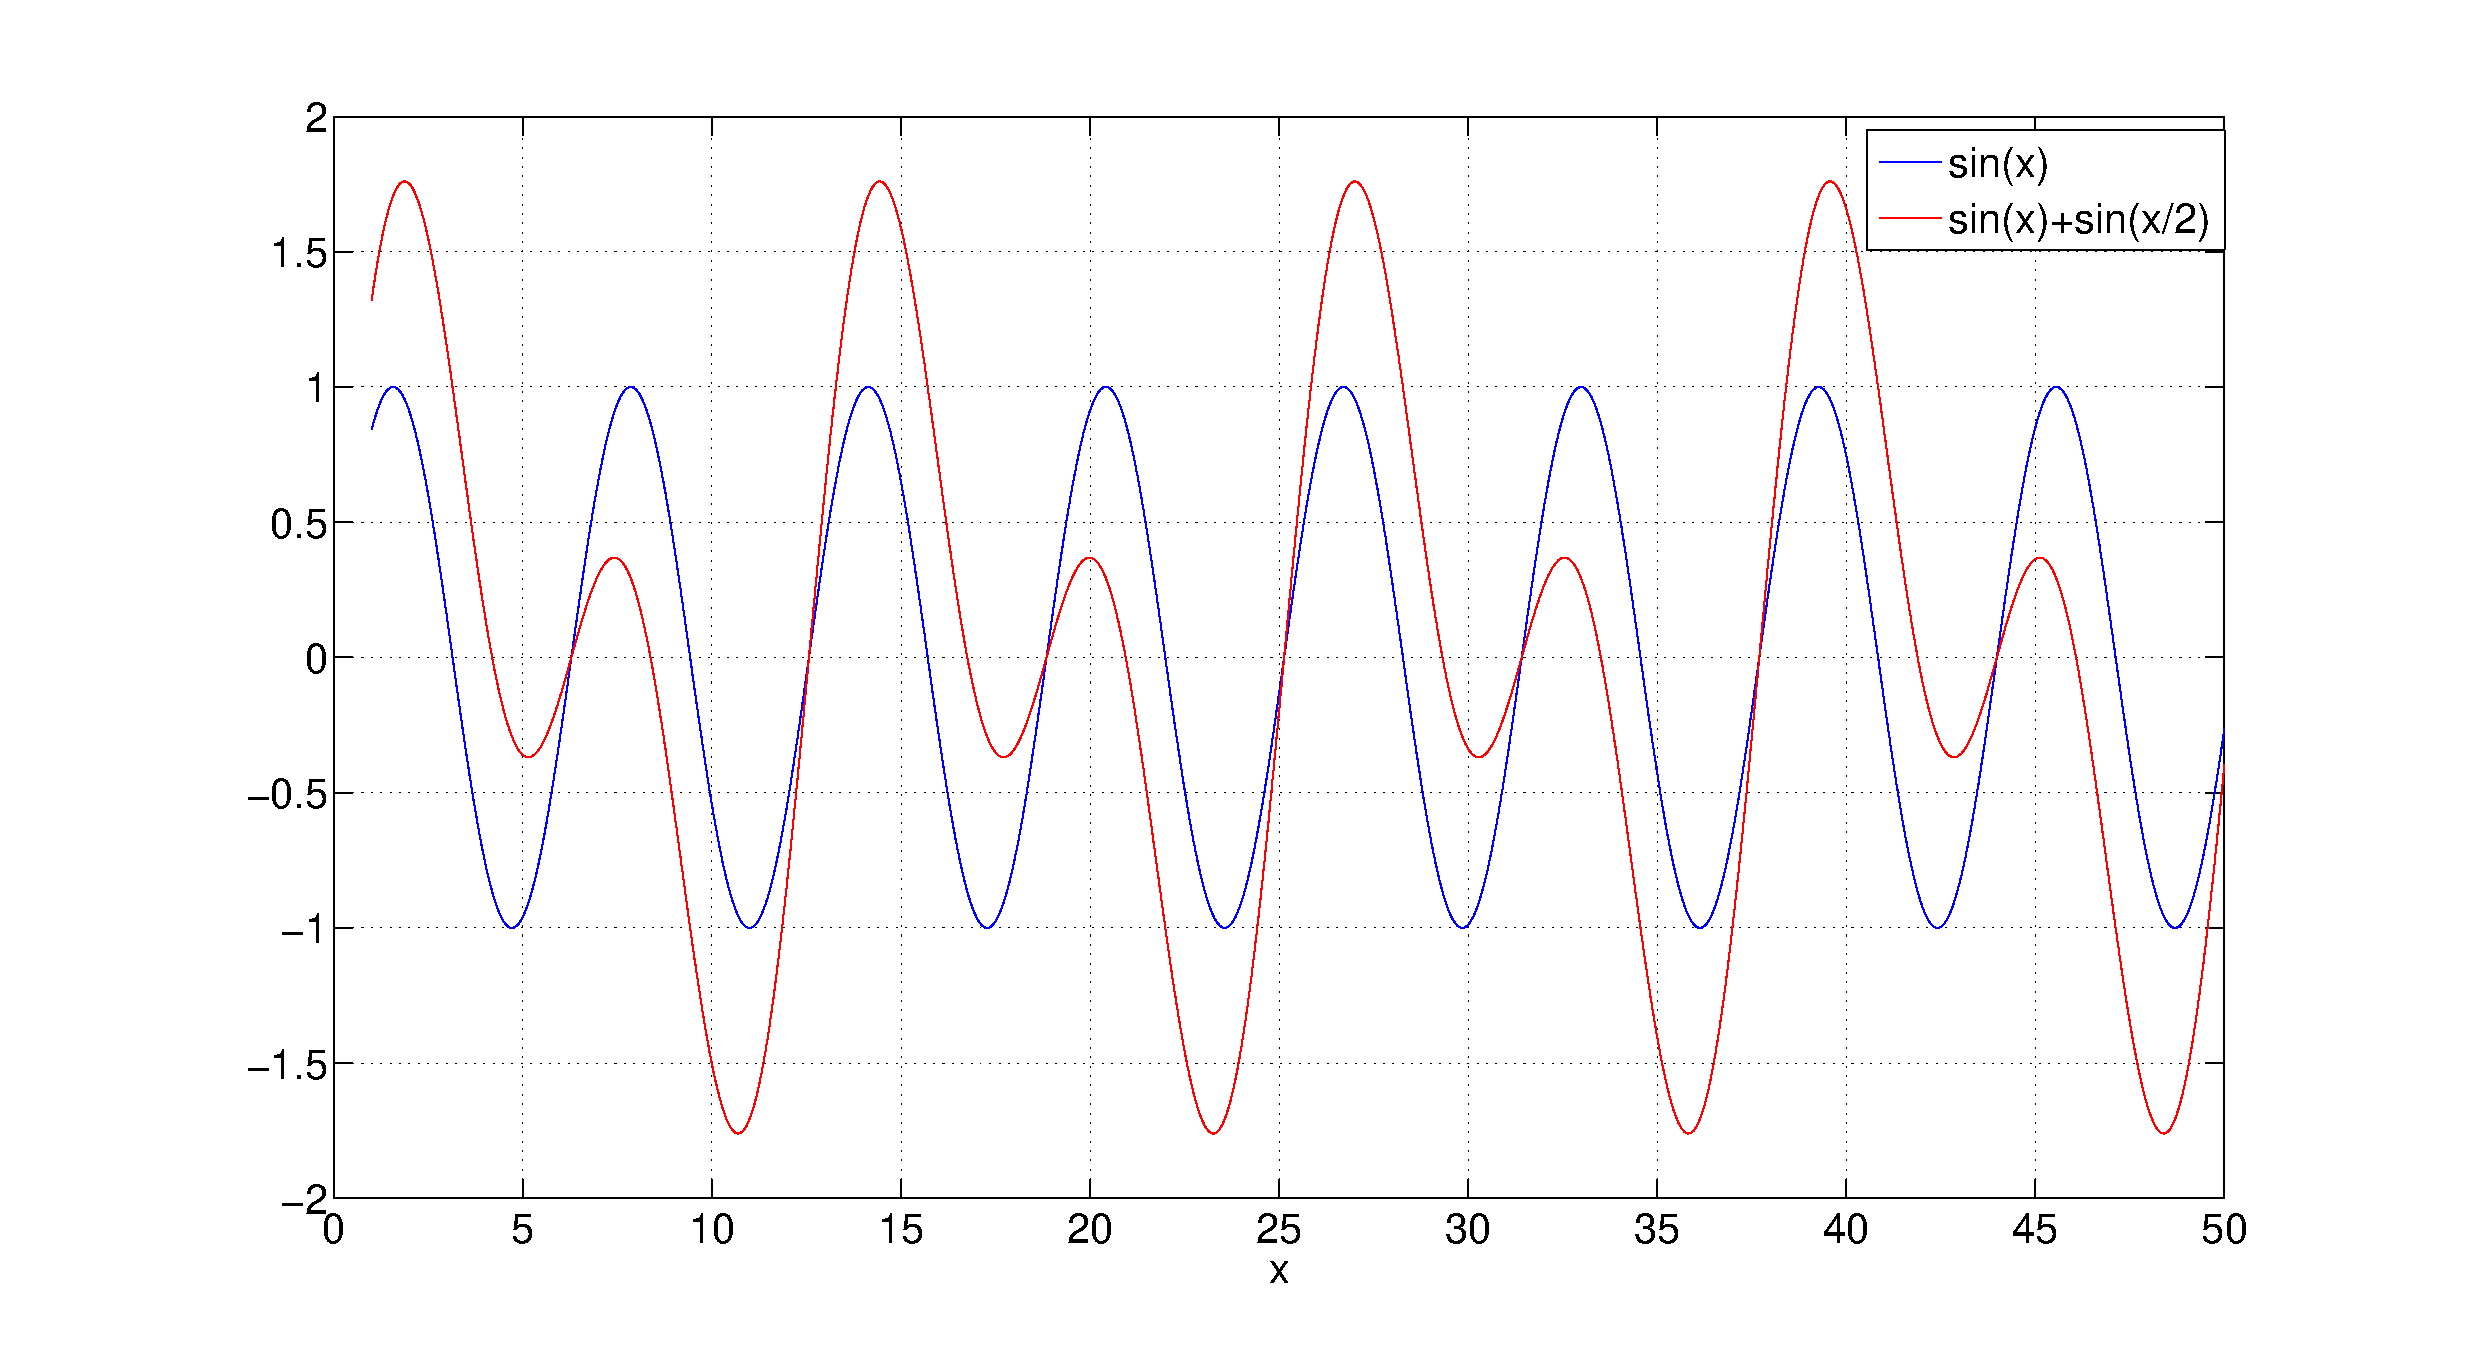
\includegraphics[scale=0.3]{period-n}
  \caption{Sinusoidal oscillations as an example of period-1~(blue) and
    period-2~(red) oscillatory dynamics.}
  \label{fig:3}
\end{figure}

The summary of all dynamical regimes detectable within the frame of the slope
algorithm goes in Tab.~\ref{tab:1}. Here we also present the numerical codes for
each possible regimes: 0 means stationary dynamics, $1\ldots n$ means
period-1$\ldots$period-$n$ oscillatory regime and $-1$ stands for the unknown or
undetermined regime.

\begin{table}[h]
  \centering
  \begin{tabular}[h]{|l|c|}
    \hline{}
    \textbf{Regime} & \textbf{Name}(\textbf{numerical code})\\
    \hline{}
    Stationary state & SS(0)\\
    \hline{}
    Period-$n$ oscillations & OS($n$) \\
    \hline{}
    Unknown/undetermined & --($-1$)\\
    \hline
  \end{tabular}
  \caption{1D dynamical regimes detected by the slope algorithm.}
  \label{tab:1}
\end{table}

\subsubsection{The slope algorithm}
\label{sec:body-slope-algorithm}

Note that the dynamics of a system cannot be stationary and non-stationary at the
same time. Thus, these two pathways of analysis are separated from each other in the
slope algorithm~(SA).

\paragraph{Stationary dynamics.}

The stationary dynamics can be easily detected when the system is already at the rest
state, meaning it does not deviate from the state significantly. This can be checked
by comparing the very last slope's amplitude to the system-wide absolute error level
(which is defined by the user). If the amplitude is so small (less than the error
level), then the decision is made right away --- \texttt{SS(0)}~(see
Tab.~\ref{tab:1}). This can be expressed by the formula:

\begin{equation}
  \label{eq:ss_abs}
  S^A_{last} < \epsilon_{abs}\,,
\end{equation}
where $S^A_{last}$ is the amplitude of the last slope in the trajectory,
i.e. containing the largest value for the time~($S^T$) of the slope. The value
of $\epsilon_{abs}$ is highly system-dependent and changes, for example, with
different units of the system. Thus, it is highly recommended to check this value
before any serious studies of the dynamics of the system of interest.

The more complex situation of the stationary dynamics detection takes place, when the
algorithm receives the time series where the system does not appear to be in its
final resting state. But, since the system has it, it must converge to it. The
convergence is manifested in the consistent decrease in the slope amplitudes when
moving from the first slopes to the last ones. So the slopes successively demonstrate
a decrease in their amplitudes as time goes on (or any other independent
variable). In this case, the SA checks the slope amplitudes moving from the last to
the first slope. If, starting from the last slope, at least 50\% (default value) of
all the amplitudes increase sequentially (in the reversed direction), then SA detects
the SS(0) regime~(Tab.~\ref{tab:1}). This increase must not be interrupted anywhere,
in other words, approximately the last half of the trajectory shows the monotonic
decay in the slope amplitudes in direct time (or other independent variable).

The tolerance $\epsilon_{rel}$ determining the criterion for the descending of the
slope amplitudes is relative and also specified by the user. Thus, the $(i+1)$
amplitude is considered to be decreasing compared to the previous $i$-th
amplitude, if the following condition is fulfilled:
\begin{equation}
  \label{eq:ss_decrease_condition}
  (S^A_{i}-S^A_{i+1}) > \epsilon_{rel}\cdot S^A_{i}
\end{equation}
This means, that from slope $i$ to slope $i+1$ the amplitude decreases for more than
$100\times\epsilon_{rel}\%$. The usual value for $\epsilon_{rel}$ is 0.01~(1\%). Note
that for the increasing amplitudes the condition cannot be ever fulfilled, since the
left hand difference of the amplitudes becomes negative in this case, while the right
hand product is always positive.

Let $M$ be the following:
\begin{equation}
  \label{eq:ss_decrease}
  M = \max\left(i\,\, |\,\, (S^A_{i}-S^A_{i+1}) \le \epsilon_{rel}\cdot S^A_{i}\right)\,|\, \left( (S^T_i < S^T_{i+1}) \,|\, (i < i+1)\right)\,,
\end{equation}
i.e. the maximum index of the slope where the
condition~(\ref{eq:ss_decrease_condition}) for the slope decrease is violated, given
that the time is always increasing in the time series (this must be applied to any
other independent variable too) and the smaller slope index corresponds to its
smaller time value.

Finally, given the total number of slope amplitudes in the simulated time series is
equal $N$, the criterion for the stationary dynamical regime is:
\begin{equation}
  \label{eq:ss_detection_condition}
  \frac{N-M}{N} > \epsilon_{thr}\,,
\end{equation}
where the $\epsilon_{thr}=0.5$~(50\%) by default and $N-M$ gives the number of slopes
sequentially decreasing at the end of the simulated time series.

Summarizing, the stationary (resting) regimes get detected in two cases:
\begin{enumerate}
\item The last amplitude is smaller than the absolute tolerance (error) given by the user.
\item At least, $100\times\epsilon_{thr}$\%~(50\%) of the slope amplitudes
  sequentially \textit{increase} as calculated \textit{from the end to the beginning}
  of the trajectory.
\end{enumerate}

For the examples of the SS detection look, for instance, into
Sections~\ref{sec:single-gene-expr} and~\ref{sec:brusselator}.

\paragraph{Non-Stationary dynamics.}

There are two ways in DINAMICA to determine the oscillatory regime of any periodicity
given the period~(return time) is constructed in a constant number of subperiods~(see
Sec.~\ref{sec:dynamical-regimes-1d}).

The \texttt{first way} to detect OS dynamics is when the system of interest is on the
attractor, that is one can find the similar slopes in the trajectory. The algorithm
here tries to find a slope that is similar (in amplitude and base) to the very last
slope of the trajectory. The comparison is made with the relative tolerance level
$\epsilon_{rel}$ that is used in the SS detection~(by decreasing slope
amplitudes). Therefore, the error level $\epsilon_{rel}$ is somewhat a demarcation
threshold between similar and different slopes. That is, the slopes are similar if
the following two criteria are fulfilled:
\begin{equation}
  \label{eq:os_similar_slopes_criteria}
  \left \{
  \begin{matrix}
    \left| S^A_i - S^A_k\right| < \epsilon_{rel}\cdot S^A_k \\
    \\
    \left| S^B_i - S^B_k\right| < \epsilon_{rel}\cdot S^A_k
  \end{matrix}
  \right.
\end{equation}
Note, that here we use the \textit{absolute} difference between the amplitude and
base values, since the approaching of the oscillatory attractor can be both from
higher slope amplitudes and lower slope amplitudes to the last one. Additionally, we
use slope bases for the comparison, since the amplitudes are not enough for the
purpose. For example, the amplitudes can be similar, but the slopes are located in
different parts of the phase space.

For the first trial of finding similar slope $k$~(see
eq.~(\ref{eq:os_similar_slopes_criteria})) takes the value of $N$~(the number of
slopes in the trajectory), while $i$ moves from $N-1$ to 1 with step 2~(since a
period is composed with 2 consecutive slopes) until the
conditions~(\ref{eq:os_similar_slopes_criteria}) are met. Once the conditions are
satisfied the algorithm proposes the lag (i.e. number of slopes in the period, see
more on the system lag in Sec.~\ref{sec:phase-test}) and decreases $k$ by one. For
every new value of $k$ algorithm tries to find the lag again to support the proposal
found for the previous value of $k$. The algorithm continues decreasing $k$ until the
newly proposed lag is not equal to the one determined for the previous $k$. The
algorithm reports how many $k$ iterations supported the first proposal of the lag,
which is the relevant information for the user.

When the lag is zero for the first value of $k$, the \texttt{second} procedure is to
be carried out. It checks for monotonic increase in the slope amplitudes as the time
goes on, in a similar way~(but with inverted conditions) the algorithm checks the
monotonic decrease in the case of SS detection.

The following condition determines the increase in the slope amplitudes:
\begin{equation}
  \label{eq:os_increase_condition}
  S^A_{i+1}-S^A_i > \epsilon_{rel}\cdot S^A_i
\end{equation}

The algorithm calculates the fraction of slopes satisfying the
condition~(\ref{eq:os_increase_condition}) at the end of the trajectory. The fraction
must be larger than the predefined error level $\epsilon_{thr}$ that is equal 0.5 by
default. Note, that this threshold error can be different from that used in the SS
detection. This is fulfilled with the set of expressions~(\ref{eq:os_increase}),
where $M$ denotes the max index of a slope where the
condition~(\ref{eq:os_increase_condition}) is violated, then the number of the
increasing slope amplitudes at the end of the trajectory equals $N-M$, where $N$ is
total number of the slopes in the trajectory. Finally, the comparison with the
threshold value is done.
\begin{equation}
  \label{eq:os_increase}
  \left \{
  \begin{matrix}
    M = \max\left(i\,\, |\,\, (S^A_{i+1}-S^A_{i}) \le \epsilon_{rel}\cdot
      S^A_{i}\right)\,|\, \left( (S^T_i < S^T_{i+1}) \,|\, (i < i+1)\right)\,, \\
    \\
    \dfrac{N-M}{N} > \epsilon_{thr}
  \end{matrix}
  \right .
\end{equation}

Summarizing, the non-stationary (oscillatory) regimes get detected in two cases:
\begin{enumerate}
\item One can find a slope similar (in amplitude and base) to the very last slope
  anywhere in the given trajectory.
\item At least, $100\times\epsilon_{thr}$\%~(50\%) of the slope amplitudes
  sequentially \textit{decrease} as calculated \textit{from the end to the beginning}
  of the trajectory.
\end{enumerate}

The examples of the OS detection can be found, for instance, in
Sections~\ref{sec:brusselator} and \ref{sec:repressilator}.


\subsubsection{General Comments on Slope Algorithm}
\label{sec:gener-comm-slope}

Here we list all the characteristics of the slope algorithm, common
pitfalls in the analysis, known problems, limitations and assumptions behind the
algorithm. Users of DINAMICA are assumed to be familiar with these notes.

\begin{enumerate}
\item The piece of the trajectory supplied to the T-system must be sufficient for the
  analysis. It also must represent the dynamics of the system under study at the most
  relevant scale.
\item The slope algorithm is a heuristic procedure, that is it detects the actual
  realized dynamics as it is provided by the user. It does not calculate any
  analytical characteristics from the rigid and solid theory to make a decision on
  the dynamics. Thus, the scope and scale of the supplied trajectories and the
  system-wide constants must be controlled by the user of the program. For example,
  the error level for the stationary dynamics detection is fully dependent on the
  system under analysis: it can be 100 or 0.0001 and only units of the model and
  common sense tell what the appropriate level is. Moreover, the part of the
  trajectory presented to the algorithm could be just a tiny piece of a larger
  picture: what if the trajectory will go extremely high with increasing slope
  amplitudes right after the time window with consistent decrease in the amplitudes?
  Such regimes do exist. This is a philosophical issue, which can be partially
  overcome with the analytical knowledge like Lyapunov exponents and linear stability
  analysis in the case of steady states. DINAMICA does NOT do this kind of
  analysis. However, the core slope algorithm can be easily extended to calculate
  analytical characteristics (like Lyapunov exponents or Floque multipliers) to
  further support the made decision. Thus, the user can do the analytical assessments
  on the steady state solutions in a separate algorithm, implemented in DINAMICA~(see
  the \texttt{(S)ingularity} menu).
\item 1D detection of the dynamics is represented with 4 distinct procedures: two for
  SS and two for OS. Given the error levels supplied by the user are set in
  correspondence with the scale of the model, the first procedures for both SS and OS
  detection methods are the most precise or, in other words, trustworthy. The second
  procedures for both SS and OS detection predict the most probable dynamical outcome
  of the model. For this reason, they produce many numerical assessment entities to
  be analyzed by the user.
\item The slope algorithm proceeds as follows. First, it tries to identify SS regime
  by the absolute tolerance way (1st procedure). If that fails, it goes for the rest
  three procedures (2nd SS and 1st and 2nd OS). The next goes the 1st OS
  procedure. If that fails, the SA proceeds to the 2nd SS procedure (identification
  of the amplitude decrease). If this does not produce any result, the algorithm
  proceeds to the 2nd OS detection procedure (monotonic increase in amplitudes).
\item OS detection relies only upon the monotonic increase (2nd procedure) in the
  slope amplitudes and not upon the decrease. However, approaching the oscillatory
  attractor can be both from the space lying outside the closed curve of the
  attractor in the phase space and from within. Thus, the decrease in the slope
  amplitudes can signify the approaching to the oscillatory attractor, but can be
  detected with 2nd SS procedure checking for the monotonic decrease in the
  amplitudes. The workaround here is the appropriate absolute error level for the SS
  detection and longer time series, since the longer time series can reveal either
  further decrease of the amplitudes or arriving to the oscillatory attractor. The
  ration between the last slope and the absolute error level is shown when SS is
  detected via the 2nd procedure. This indicates how close the final trajectory
  amplitude to the actual stationary state.
\item It is possible, given the time of the slopes, to calculate approximate rate of
  changing of the slope amplitude over time. Hence, the additional integration might
  be invoked from within the T-system to further clarify the regime, if the user has
  supplied a non-sufficient piece of the trajectory.
\end{enumerate}

\subsection{ND Dynamical Analysis}
\label{sec:nd-dynamics-analysis}

Once the slope information about each subsystem is gathered, it is supplied to the
N-dimensional algorithm. ND analysis is based on the comparison of some entities of
each system one with another so that all systems are compared. For example, if one
has three subsystems and an entity $A$ is compared, then $A_1$ is compared with
$A_2$, $A_2$ compared with $A_3$ and $A_3$ compared with $A_1$~(where $A_i$ stands
for $A$ entity in the subsystem $i$). In other words, the entity undergoes all
possible pairwise comparisons. In the system with $M$ subsystems the number of
comparisons is $M\cdot(M-1)/2$.

The comparison is made by taking the ratio between two entities being compared. The
maximal ratio out of all $M\cdot(M-1)/2$ comparisons is called \texttt{gain}. Gain is
always $\ge 1$ since the larger value is divided by the smaller one in all
comparisons unless the two comparable entities are equal.

Overall, there are two test in the ND algorithm: \texttt{homogeneity} and
\texttt{phase} tests. The former checks the levels of the variables in different
subsystems, whereas the latter checks the time moments of the slopes in order to
understand the phase shift of the subsystems in respect to each other.

The overall dynamics has its numerical code. The code is a simple average of
numerical codes of the subsystems~(see the codes in
Sec.~\ref{sec:dynamical-regimes-1d}). Thus, if all subsystems possess the same
dynamics and, hence, the same dynamical numerical code, the overall dynamical code
will be the same. If, for some reason, the numerical codes in the subsystems do not
match each other the final overall numerical code will be non-integer number
indicating the \texttt{mixed} regime. This is, in general, considered to be the error
in the dynamics checking. However, there are certain meaningful exceptions.

The preliminary test checks whether all sub-systems possess the similar dynamics. The
\texttt{mixed} regimes, i.e. when some sub-systems have one behavior, whereas others
have other behavior, are possible. In general, the mixed regimes are indicators of a
strange behavior, however, some particular examples show this type of dynamical
regime, for example, when there are two limit cycles in a systems separated in the
phase space and one of them having extremely small amplitude, thus, getting detected
as a steady state.

\subsubsection{System lag}
\label{sec:phase-test}

If all sub-systems are detected to be in one dynamical regime and this regime is not
SS, the system lag needs to be determined. The system lag is a shift between the
sub-systems as measured by the number of slopes. Practically, there are $M\cdot(M-1)/2$
comparisons in a system with $M$ sub-systems. Here, we refer to the system lag as a
maximal lag between sub-systems.

The SA utilizes the iteration procedure to go through all sub-systems. In a single
iteration, every sub-system's last slope is compared with the slopes of another
sub-system starting with the last and proceeding backwards to the first slope until
the \texttt{equal amplitude slopes} are found. Additionally, the equal amplitude
slopes must have the same direction, pointing either downwards~(descending slope) or
upwards~(ascending slope). Once these two conditions are satisfied the system lag is
reported in a number of slopes from the current one to the one having similar
slope characteristics.

The concept is further clarified by Fig.~\ref{fig:nd_lag0}. The red system $j$ runs
in synchrony with the black system $i$. So the first comparison of the amplitudes
$\left|A_0^j - A_0^i\right| < \epsilon_{rel}\cdot A_0^i$ and slopes' direction give
the positive outcome, thus, the amplitudes and directions are equal. Hence, the lag
is equal 0 and there is no need to compare other amplitudes of these two
sub-systems. The iteration switch to the next pair of sub-systems.

\begin{figure}[h]
  \centering
  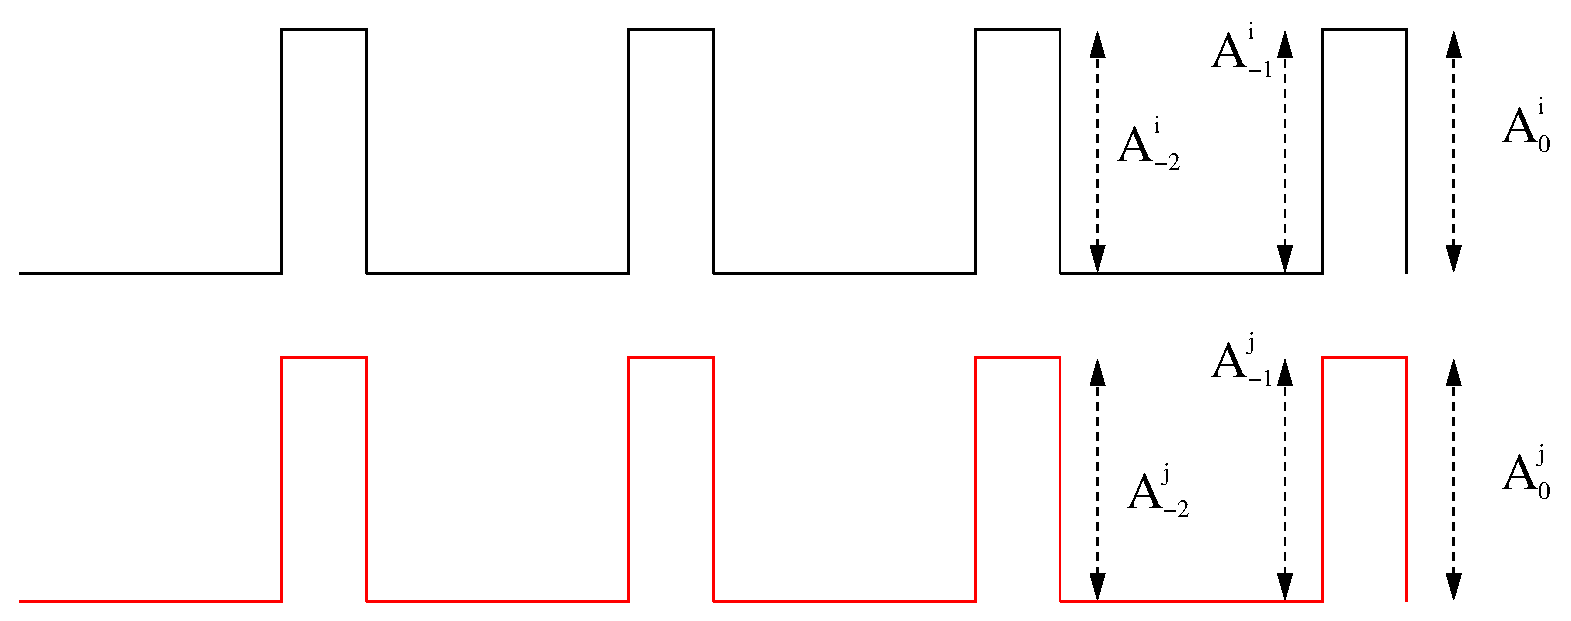
\includegraphics[scale=0.45]{nd_lag0}
  \caption{Zero system lag.}
  \label{fig:nd_lag0}
\end{figure}

If the comparison fails, the further comparisons are carried out,
i.e. $\left|A_{-1}^j - A_0^i\right| < \epsilon_{rel}\cdot A_0^i$, $\left|A_{-2}^j -
  A_0^i\right| < \epsilon_{rel}\cdot A_0^i$ etc., accompanied with similar slope
direction comparisons, until the conditions are satisfied. Note the lag is reported
as a number of slopes.

Consider the next figure~(Fig.~\ref{fig:nd_lag2}), which depicts a hypothetical
system with the system lag of 2 slopes. The inequality $\left|A_{-2}^j - A_0^i\right|
< \epsilon_{rel}\cdot A_0^i$ is fulfilled and the directions of the last slope of the
system $i$ and the slope -2 of the system $j$ coincide~(both descending).

\begin{figure}[h]
  \centering
  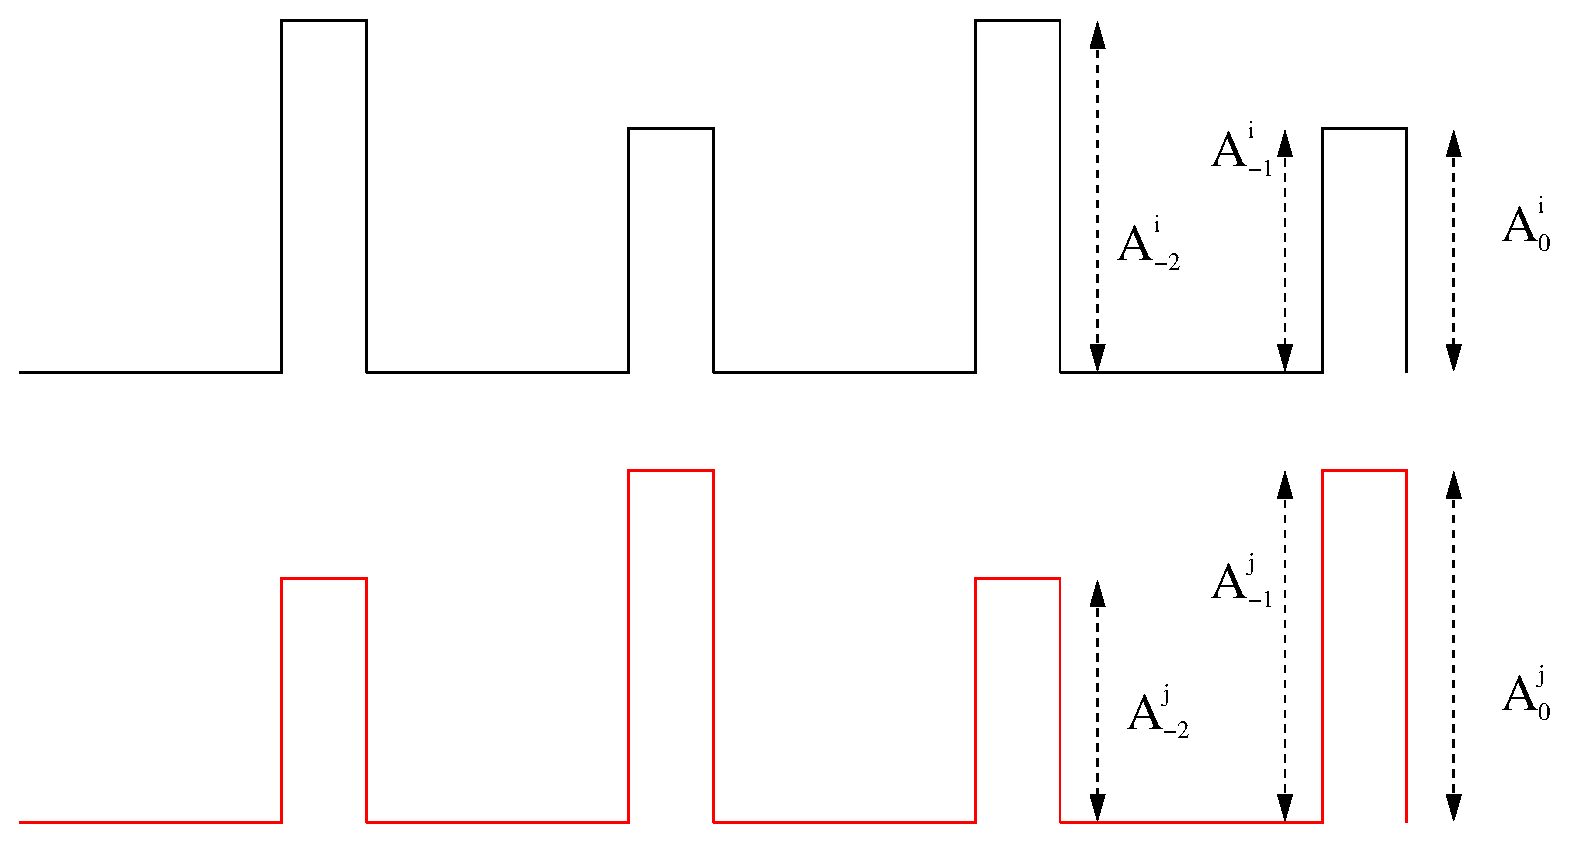
\includegraphics[scale=0.45]{nd_lag2}
  \caption{The system lag equals 2.}
  \label{fig:nd_lag2}
\end{figure}

There is an important difference between the system lag and the phase of
non-stationary dynamical regime. The phase refers to the actual time shift between
the sub-systems and determined further in the T-system using the system lag. In order
to stress the difference consider the following Fig.~\ref{fig:nd_lag0_shifted}. The
figure clearly shows the non-zero time shift between the systems, however, the system
lag is still zero.

\begin{figure}[h]
  \centering
  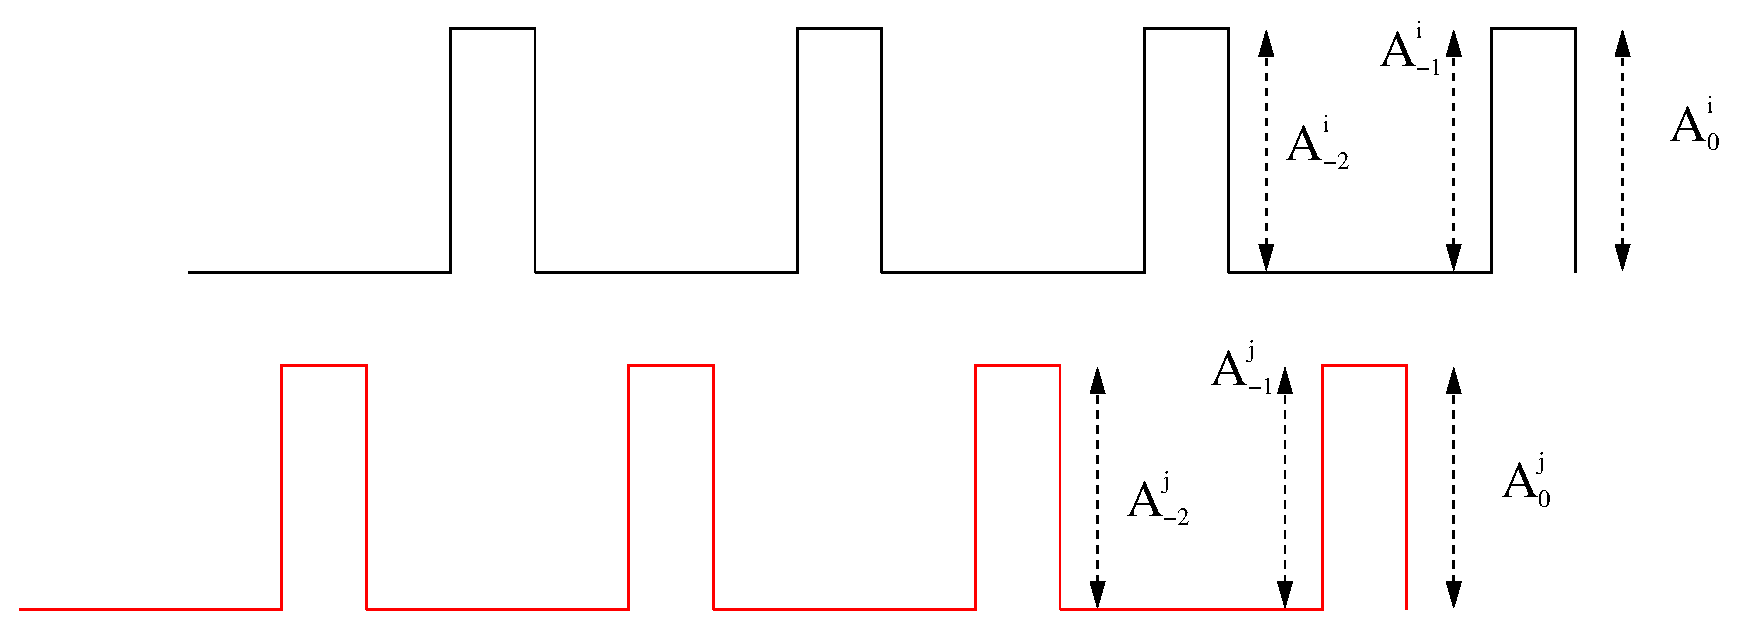
\includegraphics[scale=0.45]{nd_lag0_shifted}
  \caption{The zero lag and non-zero phase~(shifted sub-systems).}
  \label{fig:nd_lag0_shifted}
\end{figure}

Once the system lag is determined, the phase and the amplitude/base gains can be
correctly computed, since now the T-system is aware of what slopes to compare, when
calculating these entities.

\subsubsection{Phase test}
\label{sec:phase}

Phase is an actual time shift between the sub-systems. In DINAMICA it is reported as
the fraction of the period of any OS-regime. Note, that the SS regimes do not have
phase.

Given the system lag, the phase can be simply calculated as the difference of the
corresponding slopes time moments $S^{T}$. The maximal phase is reported.

If the phase shift is not zero, solution is considered to be \texttt{out-of-phase}
oscillations. Otherwise, solution is \texttt{in-phase}, meaning the synchronous
oscillations in all subsystems.

The examples shown in
Figs.~\ref{fig:nd_lag0},~\ref{fig:nd_lag2},~\ref{fig:nd_lag0_shifted} have 0T, 0.5T, and
0.5T phase shifts~(T is a period), respectively.

\subsubsection{Homogeneity test}
\label{sec:homogeneity-test}

For the homogeneity test the maximal gains of the base and amplitude are
calculated. If the base gain OR the amplitude gain is larger than $1+\epsilon_{rel}$,
then the \texttt{in-homogeneous} solution is detected. Otherwise, solution is
\texttt{homogeneous}. Note that the same $\epsilon_{rel}$ was used in the comparisons
of 1D dynamical checking algorithms.

For OS type regime the base and amplitude gains are calculated accounting for the
system lag information. For other types of dynamical behavior these gains are
calculated on the last slope amplitudes of all sub-systems.


\subsubsection{Report on the Overall Dynamics}
\label{sec:report-over-dynam}

The report of the overall dynamics of the multi-component system contains much useful
information. First, the code name for the regime comes: \texttt{SS}, \texttt{OS},
\texttt{mixed} or \texttt{-}~(undetermined) and some additional information about the
detected regimes. At the end of the report the information about homogeneity
comes. Moreover, OS regime has additional information about phase and period of
oscillations.

Here is the example of global SS detected:
\begin{verbatim}
SS(0)/IH(bg=1.12,ag=3.54)
\end{verbatim}
This means that the solution was in-homogeneous with base gain equal 1.12 and
amplitude gain equal to 3.54.

Homogeneous SS solution gets detected with the following:
\begin{verbatim}
SS(0)/H(bg=1,ag=1)
\end{verbatim}

Oscillatory regime (OS) gets detected with the following information:
\begin{verbatim}
OS-1(T=35.4)/IP(0T)/H(bg=1,ag=1)
\end{verbatim}
This indicates that the OS-1 regimes was detected with period 35.4, as determined by
simply subtracting the corresponding slopes' time moments accounting for the system
lag information. The regime happened to be the in-phase regime (IP) with maximal
phase shift of 0 periods T (0T). Finally, the homogeneity information is given.

Another type of OS detection might be:
\begin{verbatim}
OS-2(T=5.32)/OP(0.5T)/H(bg=1,ag=1)
\end{verbatim}
This means that period-2 oscillations were detected with period 5.32. The solution is
out-of-phase with the phase shift of half of the period. It is a homogeneous
solution.

The OS solution, of course, can be non-homogeneous as well. In this case, the report
would show \texttt{IH} mark with larger than 1 values of \texttt{bg}~(base gain) and/or
\texttt{ag}~(amplitude gain). 



\section{Other Dynamical Analysis Methods}
\label{sec:other-dynam-analys}




\section{Examples}
\label{sec:examples}

\subsection{Single Gene Expression}
\label{sec:single-gene-expr}

(NOTE: the ode-file of the system can be found in the package \texttt{ode/} folder
under the name \texttt{single.ode})

Here we present the simplest model representing a gene producing mRNA and, finally,
protein, which then represses its own synthesis. Formally, mRNA and protein numbers
are the only variables of the model. The ODE's representing the system are:
\begin{align}
  \label{eq:1}
  \begin{split}
    dA/dt &= \frac{\alpha}{1+\left(\frac{B}{K_h}\right)^n}-d_mA\\
    dB/dt &= gA - d_pB
  \end{split}
\end{align}


This system is merely representing self-repressing gene. The repression is carried
out through the Hill-function with a Hill-coefficient $n$. $K_h$ is affinity of the
repressor protein to the corresponding operator site of its own gene, which is
expressed as ratio between the rate constants of binding and unbinding reactions of
the repressor to/from the operator site.The mRNA and protein are degraded linearly
with rate constants $d_m$ and $d_p$, respectively. The translation process, synthesis
of the protein with the mRNA, is also linearly modelled with rate constant $g$.

For some set of the parameters one can find a stable steady state in the system. The
kinetics of the two variables of the system is depicted in Fig.~\ref{fig:single_ss}.
Being run on the trajectory, the T-system of DINAMICA reports:
\begin{verbatim}
***Checking variable a
SS(0): abs.tol = 0.001.
\end{verbatim}

This reads as follows. The T-system checked variable \texttt{a} and made a decision
on the dynamics regime~--- the steady state~(SS), as determined by the final slope
amplitude that happened to be less than the user-defined error level
\texttt{abs.tol=0.001}.

\begin{figure}[h]
  \centering
  \includegraphics[scale=0.47]{single}
  \includegraphics[scale=0.47]{single_samp}
  \caption{The time series of mRNA~($A$) and protein~($B$) of the system of a single
    self-repressing gene~(left) and the corresponding slope amplitudes as calculated
    from $A$'s trajectory~(right). Parameters used for the simulations: $\alpha =
    0.05$, $K_h = 20$, $n = 2.6$, $d_m = 0.0033$, $g = 0.1$, $d_p = 0.0033$}
\label{fig:single_ss}
\end{figure}

The result shown in Fig.~\ref{fig:single_ss} and the dynamics detected can be further
supported with the stability analysis of the fixed points of the system. This can be
done under the \texttt{Singularity} menu.
\begin{verbatim}
1) iter =   5  F(x) = -2.640e-08 0.000e+00 
Solution N 1
U(1)=1.530145
U(2)=46.368037
Analytical J=
-0.003300 -0.000255 
0.100000 -0.003300 
L_1=-0.0033 + 0.00504524i
L_2=-0.0033 + -0.00504524i
Stable
\end{verbatim}

The first line of the output shows the iteration of the algorithm at which the
solution was found and the RHS function values at the found point. It is clear that
the RHS functions are practically zeros. Thus, the algorithm indicates one solution
to be $U(1)=A=1.53$ and $U(2)=B=46.37$. Real parts of the linearized system's
eigenvalues \texttt{L\_1} and \texttt{L\_2} are negative indicating the stable steady
state. The Jacobian is also shown: \texttt{Analytical} means that the user has
supplied the Jacobian in the ode-file, while \texttt{Numerical} means that it was
computed numerically.

\subsection{Brusselator}
\label{sec:brusselator}

(NOTE: the system analyzed here is located in the package \texttt{ode/} directory
under the name \texttt{bruss.ode})

The Brusselator system is a model corresponding to a non-existing chemical system of
interaction of two molecules. Its major dynamical regime is limit-cycle oscillations.
The system of equations of the Brusselator is the following:
\begin{align}
  \label{eq:2}
  \begin{split}
    \frac{dU}{dt}&=A-(B+1)U+VU^2\\
    \frac{dV}{dt}&=BU-VU^2
  \end{split}
\end{align}

Analytically, the Hopf bifurcation at which the oscillations emerge takes place for
$B>A^2+1$, that is in this parameter region the fixed point becomes unstable. We have
shown the results of the dynamics test for parameter set: $A=1$ and $B=1.9$. This
allows having the system slowly approaching the steady
state~Fig.~\ref{fig:ss_bruss}.

Fig.~\ref{fig:ss_bruss} clearly demonstrates the consistent decrease in the slope
amplitudes leading to the steady state point of the Brusselator, which has started
from a non-resting state. The two criteria for the detection of the stationary
dynamics can be fulfilled together or one by one. Namely, the last amplitude can be
lower than the user-defined error level $\epsilon_{abs}$, indicating the steady state
or, alternatively, since all the amplitudes decrease over time, the steady state can
be detected through the second method by calculating the decrease of the slope
amplitudes.

\begin{figure}[h]
  \centering
  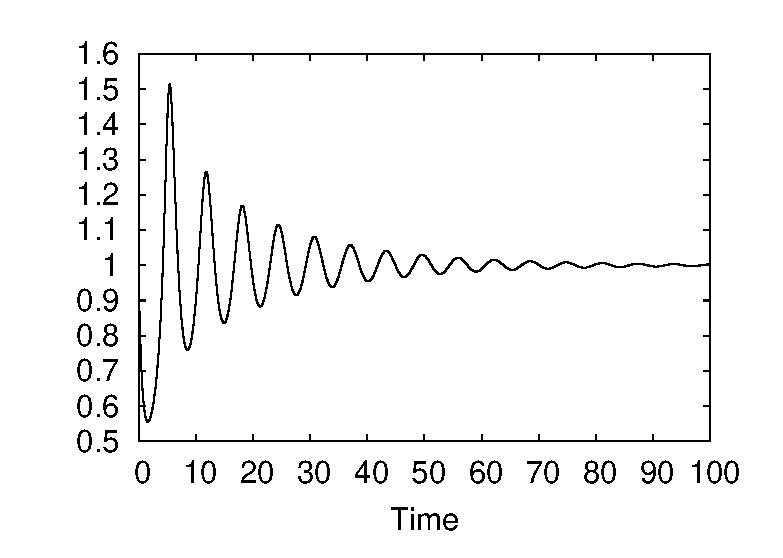
\includegraphics[scale=0.45]{sa_ex_bruss_ss}
  \includegraphics[scale=0.45]{sa_ex_bruss_ss_sl_ampl}
  \caption{The stationary dynamics of $U$ variable~(see eq.~(\ref{eq:2})) of the
    Brusselator (left) and the corresponding slope amplitudes (right) over time. The
    parameter set for the Brusselator equations: $A=1$ and $B=1.9$}
\label{fig:ss_bruss}
\end{figure}


If we make the dynamics test on the trajectory obtained from the initial conditions
$U(0)=1$ and $V(0)=1$ and total time of integration 100~(see
Fig.~\ref{fig:ss_bruss}), the DINAMICA output would be:
\begin{verbatim}
***Checking variable u
Last ampl. (0.005568) / Abs. tol. (0.001) = 5.568
SS(0): 31 of 31(100%) slopes demonstrate monotonical decrease
SS(0): total decrease=99.4198%,rel.tol=0.01
\end{verbatim}

This reads as follows. The program detected the monotonic decrease in the slope
amplitudes of the trajectory of the variable $u$. All 31 slopes demonstrate the
decrease as determined with the relative error level
\texttt{rel.tol=0.01} (1\%). Total decrease from the first slope to the last is
99.42\%. The last slope shows only 5.6 times higher amplitude than the absolute error
level \texttt{abs.tol=0.001}.

This means that the trajectory is almost at the final resting state. The SS(0) regime
is determined based on the monotonic decrease of the slope amplitudes~(the second
way). However, the ratio of the last amplitude and the absolute tolerance tells us
that the first pathway of determining SS could be reached if one had a slightly
longer integration time or a larger absolute error.

For example, if we make the absolute error at least 5.568 times larger than the
current value, e.g. abs.tol=0.006, then the SS(0) is determined by this criterion
only, like in the previous example of the single gene expression model:
\begin{verbatim}
***Checking variable u
SS(0): abs.tol = 0.006.
\end{verbatim}
Alternatively, the longer integration time would determine the SS(0) without changing
the absolute tolerance level. Since the bifurcation point leading to the oscillatory
regime is quite close to the point $A=1$ and $B=1.9$ in the parameter space, the
trajectory converge to the steady state for a quite long time for the given system.

Finally, we could set the parameters of the Brusselator system to obtain an
oscillatory dynamics. For example, $A=1$ and $B=3$ make the fixed point unstable and
oscillations emerge. The trajectory is shown on Fig.~\ref{fig:bruss_os}.

\begin{figure}[h]
  \centering
  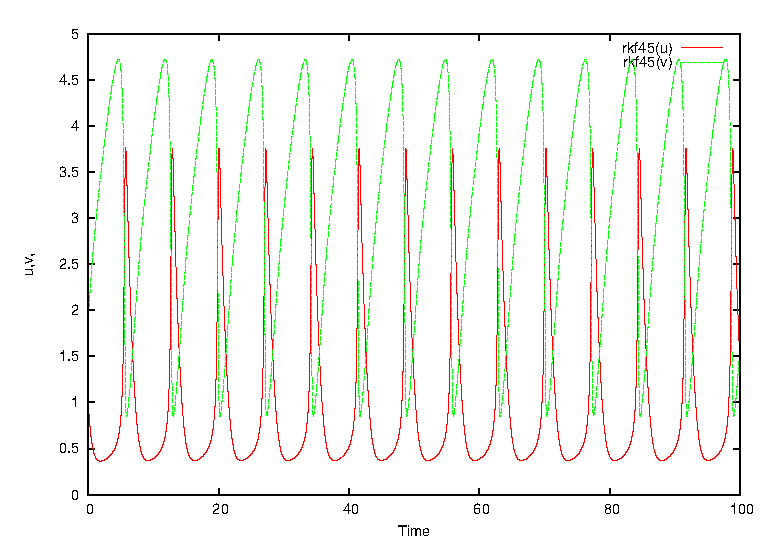
\includegraphics[scale=0.45]{sa_ex_bruss_os}
  \includegraphics[scale=0.45]{sa_ex_bruss_os_samp}
  \caption{The time series of the variables of the Brusselator~(left) for $A=1$ and
    $B=3$ and the corresponding slope amplitude values~(right).}
  \label{fig:bruss_os}
\end{figure}

The trajectory test being run on the time series shown in Fig.~\ref{fig:bruss_os}
gives the following result:
\begin{verbatim}
***Checking variable u
Lag is 1: 24 of 25 (96%) comparisons support the conclusion.
OS(1): period-1,rel.tol=0.01.
\end{verbatim}

This reads as follows. The period-1 oscillations are detected and this is supported
by the mutual comparison of 24 out of 25 slope amplitudes and slope bases. The
decision is made with the relative tolerance equal to 0.01~(1\%).

\subsection{Repressilator}
\label{sec:repressilator}

(NOTE: the file with the Repressilator system described in this section is shipped
with the package archive and located in the \texttt{ode/} directory under the name
\texttt{rep.ode})

The Repressilator is a synthetic genetic circuit consisting of three genes and
exhibiting an oscillatory behavior. The latter is possible due to the circular
arrangement of the three negative feedback loops introduced by the proteins of the
Repressilator genes. The first model of the Repressilator was proposed by the authors
who experimentally constructed the genetic
network~\cite{Elowitz2000,RepLink,RepLinkBioModels}. The system of dimensionless
ODE's is the following:
\begin{align}
  \label{eq:rep}
  \begin{split}
    da/dt &= \frac{\alpha}{1+C^n} - a \hspace{1.3cm} dA/dt = \beta(a-A)\\
    db/dt &= \frac{\alpha}{1+A^n} - b \hspace{1.3cm} dB/dt = \beta(b-B)\\
    dc/dt &= \frac{\alpha}{1+B^n} - c \hspace{1.3cm} dC/dt = \beta(c-C)\\
  \end{split}
\end{align}
The system~(\ref{eq:rep}) represents the dynamics of mRNA (lowercase letters) and
protein (uppercase letters) species of three genes A, B, and C. The repression of
each gene's mRNA is represented by the Hill function that is dependent on the
corresponding protein numbers. Additionally, each mRNA is degraded that is
represented by the negative terms of the equations. The proteins are synthesized and
degraded linearly.

The logic and the design behind the scheme imply the oscillatory behavior of the
circuit. However, there must be some steady state, which then loses stability for the
oscillations to emerge. This state appears for a small value of the transcription
rate $\alpha$. The increase in $\alpha$ makes the system lose its steady state
stability via the Hopf bifurcation and the limit cycle oscillations
emerge~Fig.~\ref{fig:rep}.

\begin{figure}[h]
  \centering
  \includegraphics[scale=0.45]{rep_ss}
  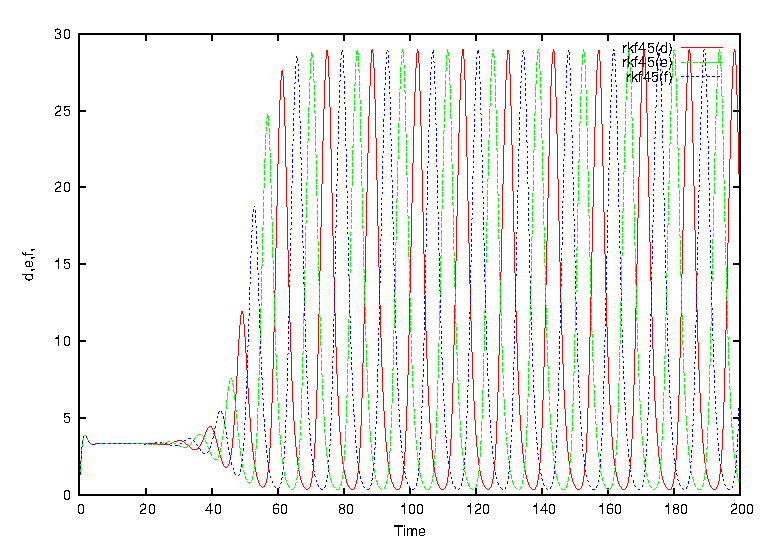
\includegraphics[scale=0.45]{rep_os}
  \caption{The stationary~(left, $\alpha=2$) and oscillatory~(right,$\alpha=40$)
    regime of the Repressilator model. The variables A, B, and C, corresponding to
    the proteins, are shown. Other parameters used in the simulation: $n=2$,
    $\beta=1$.}
\label{fig:rep}
\end{figure}

The T-system test being run on the trajectory shown in the left panel of
Fig.~\ref{fig:rep} shows SS with the absolute tolerance equal 0.001:
\begin{verbatim}
***Checking variable e
SS(0): abs.tol = 0.001.
\end{verbatim}

T-system detects the OS being run on the trajectory shown in the right panel of
Fig.~\ref{fig:rep}:
\begin{verbatim}
***Checking variable e
Lag is 1: 17 of 30 (56.6667%) comparisons support the conclusion.
OS(1): period-1,rel.tol=0.01.
\end{verbatim}

The slope amplitudes course over time clearly demonstrate how the trajectory settles
down on the limit cycle attractor. First, the amplitudes are small and then start
increasing until they end up on the plateau~(Fig.~\ref{fig:rep_samp}). Thus, the
T-system reports 17/30 amplitude comparisons to support period-1 oscillation
decision, which means that approximately half~(56.7\%) of the trajectory demonstrates
pure limit cycle oscillations. This is seen from Fig.~\ref{fig:rep_samp} where the
slope amplitudes are equal from about time 60 onward.

\begin{figure}[h]
  \centering
  \includegraphics[scale=0.7]{rep_samp}
  \caption{The slope amplitudes of the Repressilator system showing the transition to
    the oscillatory dynamics. Parameter set: $\alpha=40$, $n=2$,
    $\beta=1$~(eq.~(\ref{eq:rep})).}
  \label{fig:rep_samp}
\end{figure}

\subsection{Two coupled Brusselators}
\label{sec:two-coupl-bruss}

(NOTE: the \texttt{ode} file for the systems is called \texttt{bruss2.ode} and can be
found in the \texttt{ode/} folder of the package.)

The system of two identical diffusively coupled Brusselators gives rise to the whole
set of various dynamical behaviors. We mostly rely in our analysis
on~\cite{VolkovBruss2}, which gives the extensive bifurcation analysis of the
system. The bifurcation diagrams and results of this work can serve as a guide for
finding dynamical behaviors of the system.

The system of equations describing the behavior of coupled Brusselators is the
following:
\begin{align}
  \label{eq:bruss2}
  \begin{split}
    \frac{dx_1}{dt} &= A-(B+1)x_1+x_1^2y_1 \\
    \frac{dy_1}{dt} &= Bx_1-x_1^2y_1 + D(y_2-y_1)\\
    \frac{dx_2}{dt} &= A-(B+1)x_2+x_2^2y_2 \\
    \frac{dy_2}{dt} &= Bx_2-x_2^2y_2 + D(y_1-y_2)
  \end{split}
\end{align}

As one can see from the system~(\ref{eq:bruss2}) the coupling is realized through one
of the variables of the system $y_i$. Here we can see the 2-dimensional physical
system, each consisting with 2 variables $x_i$ and $y_i$, where $i$ refers to the
number of the system.

Given that the single Brusselator demonstrates the steady state dynamics and
oscillations appearing through the Hopf bifurcation, we can assume that the
homogeneous solutions of the systems~(\ref{eq:bruss2}) that correspond to these two
regimes must exist.

\paragraph{Homogeneous Steady State.}
\label{sec:homog-steady-stat}

For some initial conditions and parameters $A=1$, $B=1.5$, and $D=0.57$ the
system~(\ref{eq:bruss2}) converges to a steady state~Fig.~\ref{fig:br2_hss}.

\begin{figure}[h]
  \centering
  \includegraphics[scale=0.65]{br2_hss}
  \caption{The steady state of the system~(\ref{eq:bruss2}). Parameters: $A=1$,
    $B=1.5$, $D=0.57$. The initial condition for the simulation was: $x_1=10$,
    $y_1=1.5$, $x_2=1$, $y_2=15$.}
  \label{fig:br2_hss}
\end{figure}

The T-system of DINAMICA reports:
\begin{verbatim}
***Checking sub-system 1(u1):
SS(0): abs.tol = 0.001.

***Checking sub-system 2(u2):
SS(0): abs.tol = 0.001.
========
DYNAMICS:
SS(0)/H(bg=1,ag=1)
\end{verbatim}

So, the both subsystems were determined to have SS(0) and the total regime is
\texttt{homogeneous} SS(0). The overall report on the system can be seen under the
title \texttt{DYNAMICS:}. Homogeneity is seen by amplitude~(\texttt{ag}) and
base~(\texttt{bg}) gains both equal to 1~(about the base and amplitude gains see the
Section~\ref{sec:nd-dynamics-analysis}).

\paragraph{Homogeneous In-Phase Oscillations.}
\label{sec:homog-phase-oscill}

Increasing parameter $B$ to 2.5 and starting from the steady state obtained in the
previous section as the initial condition, one can see the synchronous oscillatory
dynamics of the system~(\ref{eq:bruss2}). The solution is shown in
Fig.~\ref{fig:br2_hos}.

\begin{figure}[h]
  \centering
  \includegraphics[scale=0.65]{br2_hos}
  \caption{The synchronous oscillatory solution of system of
    eqs.~(\ref{eq:bruss2}). Parameter used in simulation: $A=1$, $B=2.5$,
    $D=0.57$. The initial condition was the steady state obtained in the
    previous section.}
  \label{fig:br2_hos}
\end{figure}

The T-system of DINAMICA reports:
\begin{verbatim}
***Checking sub-system 1(u1):
Lag is 1: 25 of 27 (92.5926%) comparisons support the conclusion.
OS(1): period-1,rel.tol=0.01.

***Checking sub-system 2(u2):
Lag is 1: 25 of 27 (92.5926%) comparisons support the conclusion.
OS(1): period-1,rel.tol=0.01.
========
DYNAMICS:
OS-1(T=6.591)/IP(0T)/H(bg=1,ag=1)
\end{verbatim}

The report reads as follows. Each subsystem has been determined to have period-1
oscillations, i.e. OS(1), with the relative error equal to 1\%. More than 92\% of the
slope comparisons support the period-1 conclusion for both sub-systems. Thus, it is
believed to be true single period oscillations. The overall dynamics checking does
not reject the subsystem's conclusions about the regime and furthermore shows that
the solution is synchronous~(in-phase, \texttt{IP}) with period equal to 6.591 and 0
phase shift~(\texttt{0T}) as measured in the period units. Moreover, the regime is
homogeneous: amplitude and base gains are both equal to 1.

\paragraph{In-homogeneous Steady State.}
\label{sec:homog-steady-state}

The work~\cite{VolkovBruss2} reports that for the IP solution parameter set we used
in the previous section, i.e. $A=1$, $B=2.5$, $D=0.57$, there is another stable
solution that is in-homogeneous steady state.

Here, in order to find the unstable solution, we will use the random initial
condition approach, which is an additional technique utilized by the T-system of
DINAMICA. The random initial condition technique assigns random initial conditions
and tries out the trajectory. This method is available under the DINAMICA's
\texttt{R(a)ndom} menu.

Here, we opted to throw 10 random initial conditions for the system~(\ref{eq:bruss2})
with the span equal to 10~(for more details about the random initial conditions see
the appropriate section of the DINAMICA's manual) that was found to be
sufficient. For each initial condition T-system performs the dynamical test and
reports the result for every such test as well as the overall statistics at the end
of the calculation. Additionally the analyzed trajectories are plotted. This
example's plot can be seen in Fig.~\ref{fig:bruss2_rnd_trials}.

\begin{figure}[h]
  \centering
  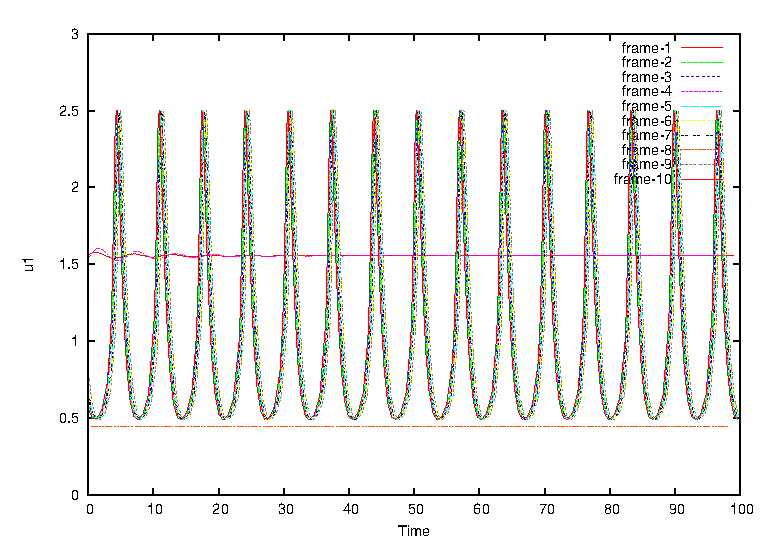
\includegraphics[scale=0.75]{br2_rnd}
  \caption{The output of the random initial condition trials. 10 random trials are
    plotted for the parameter set: $A=1$, $B=2.5$, and $D=0.57$.}
  \label{fig:bruss2_rnd_trials}
\end{figure}

The report looks as following:
\begin{verbatim}
Dynamics report:
#1) OS-1(T=6.5894)/IP(0T)/H(bg=1,ag=1)
#2) SS(0)//IH(bg=1.53092,ag=2.38667)
#3) OS-1(T=6.5628)/IP(0T)/H(bg=1,ag=1)
#4) SS(0)//IH(bg=1.53091,ag=1.59574)
#5) OS-1(T=6.5888)/IP(0T)/H(bg=1,ag=1)
#6) OS-2(T=13.0331)/IP(0T)/H(bg=1,ag=1)
#7) OS-1(T=6.5762)/IP(0T)/H(bg=1,ag=1)
#8) OS-1(T=6.5635)/IP(0T)/H(bg=1,ag=1)
#9) SS(0)//IH(bg=1.53093,ag=2.63333)
#10) OS-1(T=6.6523)/IP(0T)/H(bg=1,ag=1)
Abs.tol = 0.001, rel.tol = 0.01
-------------------
Regimes statistics:
-------------------
Number of regimes: 10
Steady States: 3 (30%)
Oscillatory: 7 (70%)
Homogeneous: 7 (70%)
In-homogeneous: 3 (30%)
Homogeneous oscillatory: 7 (70%, 100% of homogeneous)
In-homogeneous oscillatory: 0 (0%, 0% of in-homogeneous)
In-phase oscillatory: 7 (70%, 100% of oscillatory)
Out-of-phase oscillatory: 0 (0%, 0% of oscillatory)
Mixed: 0 (0%)
Undetermined: 0 (0%)
\end{verbatim}

One can see both from the report and from the output
figure~(Fig.~\ref{fig:bruss2_rnd_trials}) that the system has determined two stable
dynamical regimes: in-phase oscillatory and in-homogeneous steady state. The latter
is characterized with different steady state levels of the subsystems in the phase
space. For example, the second solution in the report shows the base gain equal to
around 1.5 meaning that the levels of the last slopes in the two subsystems differ:
one level is 1.5 times higher than the other. Note, that the amplitude gain for the
SS comparisons is not important, since the steady state level amplitudes eventually
have to approach, by the definition, an infinitesimal value.  Finally, the
statistics is shown, where different kinds of comparisons are brought together to
exemplify the diversity of behaviors of the system under study.

\paragraph{Out-of-phase oscillations.}
\label{sec:out-phase-oscill}

According to~\cite{VolkovBruss2} for $A=2$, $B=7$ and $D=0.24$ the system of two
coupled Brusselators contain the out-of-phase oscillation with half a period phase
shift. In order to find the solution we resort to the same random initial condition
technique as in the previous section, since the solution co-exist with the in-phase
oscillations. The result is shown in Fig.~\ref{fig:br2_rnd_op}, where only three
trial results are given: one in-phase and two out-of-phase oscillatory regimes.

\begin{figure}[h]
  \centering
  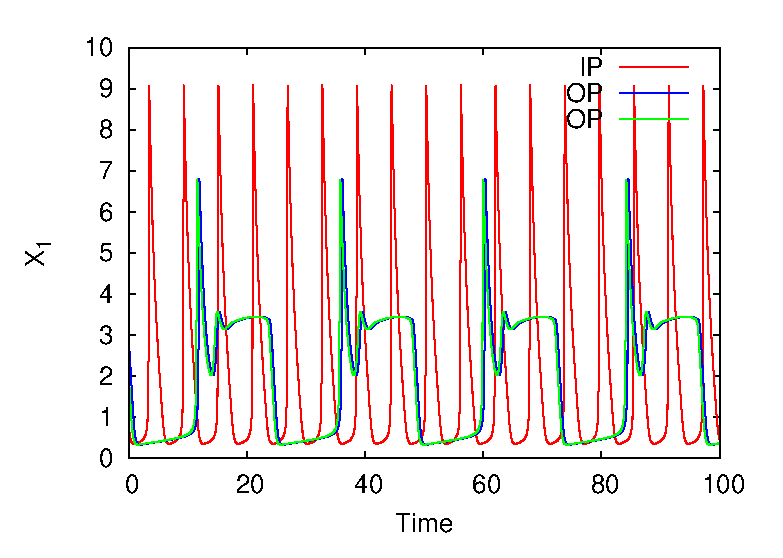
\includegraphics[scale=0.45]{br2_rnd_op}
  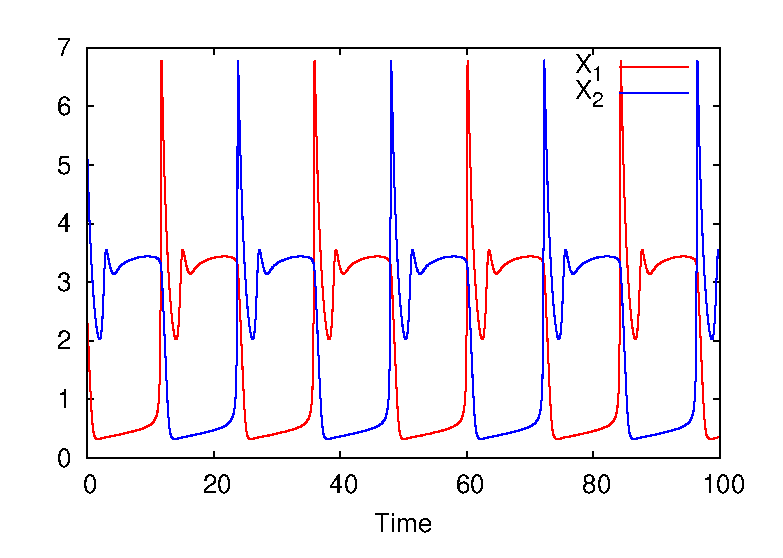
\includegraphics[scale=0.45]{br2_op}
  \caption{The random initial conditions to find the out-of-phase oscillations. Left:
    only three trials are shown giving in-phase~(IP) and two out-of-phase~(OP)
    trajectories. Right: out-of-phase solution with half of the period phase
    shift. Parameters for the system~(\ref{eq:bruss2}): $A=2$, $B=7$, and $D=0.24$. }
  \label{fig:br2_rnd_op}
\end{figure}


The dynamical test for the 10 random trials results in:
\begin{verbatim}
Dynamics report:
#1) OS-1(T=5.86)/IP(0T)/H(bg=1,ag=1)
#2) OS-1(T=5.86)/IP(0T)/H(bg=1,ag=1)
#3) OS-1(T=5.86)/IP(0T)/H(bg=1,ag=1)
#4) OS-1(T=5.86)/IP(0T)/H(bg=1,ag=1)
#5) OS-4(T=24.198)/OP(0.499959T)/H(bg=1,ag=1.00012)
#6) OS-4(T=24.198)/OP(0.499959T)/H(bg=1,ag=1.00008)
#7) OS-1(T=5.86)/IP(0T)/H(bg=1,ag=1)
#8) OS-1(T=5.86)/IP(0T)/H(bg=1,ag=1)
#9) OS-1(T=5.86)/IP(0T)/H(bg=1,ag=1)
#10) OS-1(T=5.86)/IP(0T)/H(bg=1,ag=1)
Abs.tol = 0.001, rel.tol = 0.01
-------------------
Regimes statistics:
-------------------
Number of regimes: 10
Steady States: 0 (0%)
Oscillatory: 10 (100%)
Homogeneous: 10 (100%)
In-homogeneous: 0 (0%)
Homogeneous oscillatory: 10 (100%, 100% of homogeneous)
In-homogeneous oscillatory: 0 (0%, NAN% of in-homogeneous)
In-phase oscillatory: 8 (80%, 80% of oscillatory)
Out-of-phase oscillatory: 2 (20%, 20% of oscillatory)
Mixed: 0 (0%)
Undetermined: 0 (0%)
\end{verbatim}

From the reports it is easy to see that there were found 2 OS-4 dynamical regimes
(\#5 and \#6) with period of 24.2. These oscillatory behaviors are classified as the
homogeneous out-of-phase oscillations with phase shift of approximately half of the
period. All other 8 trials gave the normal homogeneous in-phase oscillations.

Fig.~\ref{fig:br2_rnd_op} clearly shows the curly shape of the out-of-phase
oscillations. There are 4 subperiods for the oscillatory trend. Although it cannot be
clearly discerned from the figure, the 4-th subperiod contains practically small
slopes in it.

\paragraph{In-homogeneous oscillations.}
\label{sec:homog-oscill}

The system~(\ref{eq:bruss2}) of two coupled Brusselators comprise one more
interesting dynamical regime, that is in-homogeneous oscillations. The general
characteristic of the behavior is the different levels of oscillations in the
sub-systems. It usually takes place when the Hopf bifurcation appears on the
in-homogeneous steady state solutions. The waveform of the in-homogeneous OS for the
system~(\ref{eq:bruss2}) is shown in Fig.~\ref{fig:br2_ihos}.

\begin{figure}[h]
  \centering
  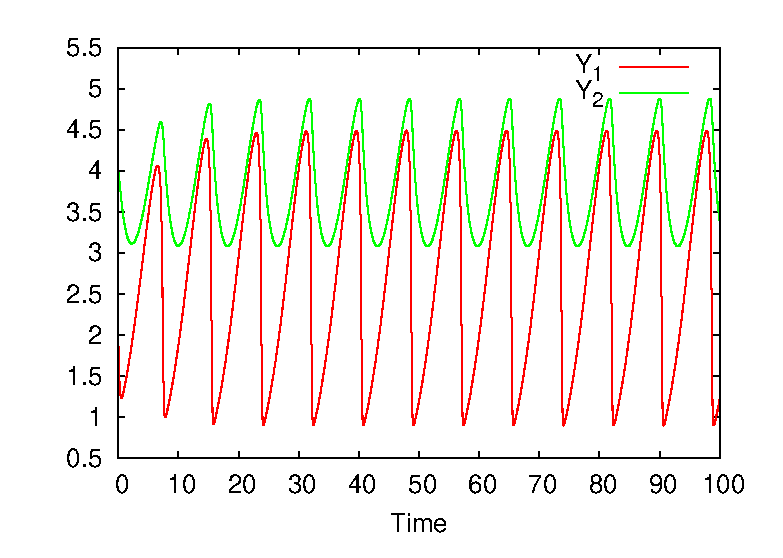
\includegraphics[scale=0.65]{br2_ihos}
  \caption{The in-homogeneous oscillatory solution of two coupled
    Brusselators. Parameters: $A=1$, $B=3.2$, $D=0.57$.}
  \label{fig:br2_ihos}
\end{figure}

The trajectory shown in Fig.~\ref{fig:br2_ihos} is analyzed by T-system of DINAMICA
giving the following output:
\begin{verbatim}
***Checking sub-system 1(y1):
# subperiods is 1: 18 of 22 (81.8182%) comparisons support the conclusion.
OS(1): period-1,rel.tol=0.01.

***Checking sub-system 2(y2):
# subperiods is 1: 17 of 21 (80.9524%) comparisons support the conclusion.
OS(1): period-1,rel.tol=0.01.

Could not determine the lag[0] => IH?
#0) Systems lag = -1
========
DYNAMICS:
OS-1(T=8.322)/OP(-1T)/IH(bg=3.43325,ag=1.99052)
\end{verbatim}

T-system has checked the first sub-system~(on the variable $y_1$) and reported about
OS-1 regime found. Similarly, for the second sub-systems~($y_2$). Finally, the lag
between the two sub-systems could not be found due to the inhomogeneity of the
two. Thus, the system lag is set to be -1 as a convention for the not-found
lag.

Additionally, in-homogeneous oscillatory solutions cannot be determined to have a
phase shift one from another. Hence, the T-system uses conventionally the negative
number~(usually close to -1) for the phase shift of such dynamical behaviors. However,
the base and amplitude gains can be well determined and they are reported.

\subsection{Three coupled Brusselators}
\label{sec:three-coupl-bruss}

(NOTE: the three coupled Brusselators system is defined in \texttt{bruss3.ode} file
of the package and can be found in \texttt{ode/} folder.)

Here we consider another example of coupled Brusselators, where the coupling is
carried out through the common media via the slow variable $y_i$ and three
oscillators are coupled. In general, this type of the system does not differ from the
previously considered 2 Brusselators, except for the number of them, since the
system~(\ref{eq:bruss2}) can be brought to the form of the following system:
\begin{align}
  \label{eq:bruss3}
  \begin{split}
    \frac{dx_i}{dt} &= A-(B+1)x_i+x_i^2y_i \\
    \frac{dy_i}{dt} &= Bx_i-x_i^2y_i + D(\frac{1}{N}\sum\limits_{j=1}^Ny_j-y_i)\\
  \end{split}
\end{align}

Eq.~(\ref{eq:bruss3}) represents the dynamical system of a single $i$-th oscillator,
where the total number of oscillators $N=3$. This system is known to have so called
``wave'' solution where the trajectory is a period-2 oscillation for each of the
oscillators and the phase shift between the oscillators is
$T/3$~(Fig.~\ref{fig:br3_wave}).

\begin{figure}[h]
  \centering
  \includegraphics[scale=0.6]{br3_wave}
  \caption{The so called "wave" solution to the eq.~(\ref{eq:bruss3}). Parameters used:
    $A=1$, $B=15.4$, $D=0.046$.}
\label{fig:br3_wave}
\end{figure}

T-system reports on the ``wave'' solution~(as shown in Fig.~\ref{fig:br3_wave}, but
with time 1000):
\begin{verbatim}
***Checking sub-system 1(y1):
# subperiods is 2: 42 of 49 (85.7143%) comparisons support the conclusion.
OS(2): period-2,rel.tol=0.01.

***Checking sub-system 2(y2):
# subperiods is 2: 42 of 49 (85.7143%) comparisons support the conclusion.
OS(2): period-2,rel.tol=0.01.

***Checking sub-system 3(y3):
# subperiods is 2: 46 of 49 (93.8776%) comparisons support the conclusion.
OS(2): period-2,rel.tol=0.01.

period 1: 76.766 = 25.38 + 51.386
period 2: 76.889 = 25.43 + 51.459
period 3: 76.848 = 51.445 + 25.403
phase shift 1: 0.334341
phase shift 2: 0.332856
phase shift 3: 0.667018
========
DYNAMICS:
OS-2(T=76.766)/OP(0.666662T)/H(bg=1.00006,ag=1.00007)
\end{verbatim}

The report above reads as follows. Each sub-system was determined to have OS-2
periodic trajectory. Periods of each of the sub-system were about 76.8, divided into
two subperiods: 25.4 and 51.4. Phase shifts  were 0.33, 0.33 and 0.67. The first two
are expected phase shifts as was noted above for the ``wave'' trajectory, however,
0.67 phase shift is also reported, for the mutual comparison is carried out between
\textbf{all} possible pairs of oscillators, and, of course, there is a pair of
oscillators that has a phase shift of double of the minimal one 0.33.

In general, this is the case for N oscillators' system with equal phase shift between
the ``closest'' oscillators, i.e. system is symmetric with regards to the phase
shift. The minimal phase shift is going to represent this ``closest'' components and
there will be also phase shifts of i$\times$ minimal-phase-shift, where i runs from 1
to $N-1$.

Another example of the phase symmetric oscillations but with different periodicity
inside each oscillator is shown in Fig.~\ref{fig:br3_os3}.

\begin{figure}[h]
  \centering
  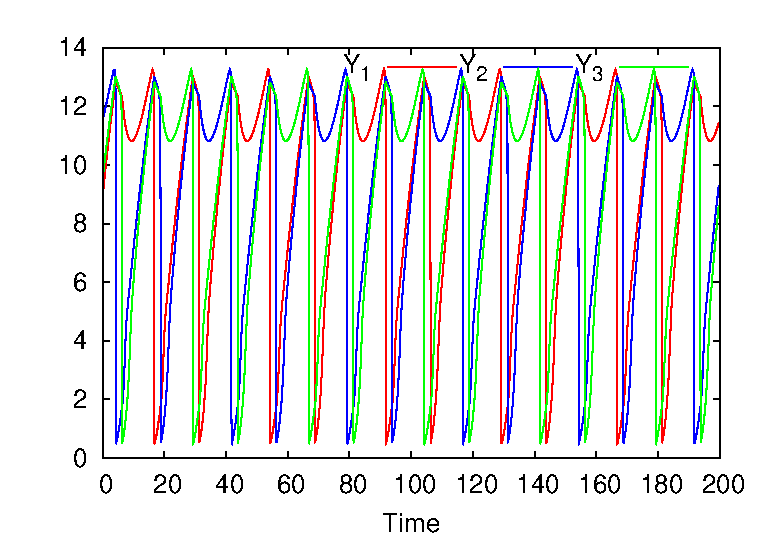
\includegraphics[scale=0.6]{br3_os3}
  \caption{The OS-3 solution with T/3 phase shift. Parameters: $A=1$, $B=6$, $D=0.234$}
  \label{fig:br3_os3}
\end{figure}

The shown in Fig.~\ref{fig:br3_os3} regime is OS-3 oscillations as T-system reports:
\begin{verbatim}
***Checking sub-system 1(y1):
# subperiods is 3: 24 of 29 (82.7586%) comparisons support the conclusion.
OS(3): period-3,rel.tol=0.01.

***Checking sub-system 2(y2):
# subperiods is 3: 24 of 29 (82.7586%) comparisons support the conclusion.
OS(3): period-3,rel.tol=0.01.

***Checking sub-system 3(y3):
# subperiods is 3: 24 of 29 (82.7586%) comparisons support the conclusion.
OS(3): period-3,rel.tol=0.01.

period 1: 37.493 = 12.498 + 13.05 + 11.945
period 2: 37.498 = 11.946 + 12.497 + 13.055
period 3: 37.493 = 13.055 + 11.94 + 12.498
phase shift 1: 0.333342
phase shift 2: 0.666569
phase shift 3: 0.333476
========
DYNAMICS:
OS-3(T=37.493)/OP(0.666569T)/H(bg=1.00001,ag=1.00008)
\end{verbatim}

Again, one can see the 0.33 to be the minimal phase shift between the oscillators,
but the period is now composed of 3 subperiods, which is reliably determined for each
of the sub-systems.

All regimes demonstrated in this section are homogeneous.

\subsection{Two coupled genetic Repressilators}
\label{sec:two-coupled-genetic}

(NOTE: the two coupled Repressilators system can be found in \texttt{repB2.ode} under
the \texttt{ode/} directory of the package.)

Recent example of the genetic dynamical system possessing a multitude of dynamical
behaviors has been reported in~\cite{Ullner2007}. The system is a further development
of the original Repressilator system~(see eq.~(\ref{eq:rep}) and~\cite{Elowitz2000})
and contains the following equations~\cite{Ullner2007,Ullner2008,Garcia2004}:
\begin{align}
  \label{eq:repB2}
  \begin{split}
    \dfrac{da_i}{dt} &= \dfrac{\alpha}{1+C_i^n} - a_i \hspace{3.1cm} \dfrac{dA_i}{dt} = \beta_a(a_i-A_i)\\
    \dfrac{db_i}{dt} &= \dfrac{\alpha}{1+A_i^n} - b_i \hspace{3.1cm} \dfrac{dB_i}{dt} = \beta_b(b_i-B_i)\\
    \dfrac{dc_i}{dt} &= \dfrac{\alpha}{1+B_i^n} - c_i + \kappa\frac{S_i}{1+S_i} \hspace{1.3cm} \dfrac{dC_i}{dt} = \beta_c(c_i-C_i)\\
  \end{split}
\end{align}
\begin{equation}
  \notag
  \dfrac{dS_i}{dt} = -k_{s0}S_i + k_{s1}B_i - \eta(S_i - Q\bar S)\,,
\end{equation}
where $\bar S = \dfrac{1}{N}\sum\limits_{j=1}^NS_j$~($N$ is the number of
oscillators).

The system~(\ref{eq:repB2}) has the original Repressilator's three genes augmented
with a small diffusive molecule carrying out the coupling function. The molecule is
represented by the term $S_i$ and affects the expression rate of the mRNA $c_i$. The
coupling itself is realized through the diffusion of $S_i$. Furthermore, the
contribution of all Repressilator cells is represented by the average concentration
of $S_i$ molecules $\bar S$ in all cells, thus, having an assumption of fast mixing
of $S$ molecules in the media. Since the mechanism is borrowed from a clear natural
example of so called quorum sensing found in bacteria, the average concentration of
$S$ molecules is further multiplied with the quorum sensing coefficient $Q$ that
takes the values from the interval $[0,1]$. The $Q$ parameter determines how close
the cells are in the media. For example, if $Q=1$ all cells are tightly connected and
once $S$ molecule is produced in cell $i$ it is immediately available to all other
cells. On the contrary, $Q=0$ indicates the full dilution of $S$ molecules in the
media, i.e. cells are far away from each other. For further details,
see~\cite{Ullner2008}.

There is a whole set of the dynamical behaviors the model demonstrates, e.g. as the
quorum sensing parameter $Q$ varies. We will follow the results reported
in~\cite{Ullner2008}. Until a further notice made, the default parameter set we use
is: $N=2$, $\alpha=216$, $n=2.6$, $\beta_a=0.85$, $\beta_b=0.1$, $\beta_c=0.1$,
$\kappa=25$, $k_{s0}=1$, $k_{s1}=0.01$, $\eta=2$ and we vary $Q$ in the range $[0, 1]$.

\paragraph{Anti-phase oscillations.}
\label{sec:anti-phase-oscill}

The only pure oscillatory regime the system~(\ref{eq:repB2}) has is the anti-phase
oscillations, i.e. oscillations with phase shift of half a period. So, given the
default parameter set and $Q=0.1$ we observe the anti-phase
kinetics~(Fig.~\ref{fig:rB2_op}).

\begin{figure}[h]
  \centering
  \includegraphics[scale=0.65]{rB2_op}
  \caption{The anti-phase solution of the system~(\ref{eq:repB2}). The default
    parameter set and $Q=0.1$.}
  \label{fig:rB2_op}
\end{figure}

The T-system being run on the results shown in Fig.~\ref{fig:rB2_op} reports:
\begin{verbatim}
***Checking sub-system 1(a1):
# subperiods is 1: 16 of 17 (94.1176%) comparisons support the conclusion.
OS(1): period-1,rel.tol=0.01.

***Checking sub-system 2(a2):
# subperiods is 1: 15 of 16 (93.75%) comparisons support the conclusion.
OS(1): period-1,rel.tol=0.01.

DYNAMICS:
OS-1(T=51.08)/OP(0.5T)/H(bg=1,ag=1)
\end{verbatim}

The above report shows the homogeneous oscillations with phase shift of 0.5 of the
period, that is 51.08. Both sub-systems are reported to have OS-1 regime.

\paragraph{Oscillations co-exist with homogeneous steady state.}
\label{sec:oscill-co-exist}

If we set $Q=0.2$ the dynamical picture of the system changes and new dynamics
emerge. Namely, the stable homogeneous steady state solution in addition to the
oscillatory anti-phase solution.

Let us try to identify the solution using the random initial conditions. In the
following we opted to have 300 randomly thrown initial points for simulations:
\begin{verbatim}
Abs.tol = 0.001, rel.tol = 0.01
-------------------
Regimes statistics:
-------------------
Number of regimes: 300
Steady States: 298 (99.3333%)
Oscillatory: 2 (0.666667%)
	Periodicity (unique): 1
Homogeneous steady state: 298 (99.3333%)
In-homogeneous steady state: 0 (0%)
Homogeneous oscillatory: 2 (0.666667%, 0.666667% of homogeneous)
In-homogeneous oscillatory: 0 (0%, NAN% of in-homogeneous)
In-phase oscillatory: 0 (0%, 0% of oscillatory)
Out-of-phase oscillatory: 2 (0.666667%, 100% of oscillatory)
Mixed: 0 (0%)
Undetermined: 0 (0%)
\end{verbatim}

So the homogeneous steady state is a dominant regime (with the throwing radius of
200) with 298 appearances, whereas the anti-phase solution appeared only twice. The
report also specified the solutions found:
\begin{verbatim}
...
#228) SS(0)/H(bg=1,ag=1)
#229) OS-1(T=49.381)/OP(0.500142T)/H(bg=1.00007,ag=1)
...
\end{verbatim}

Thus, the same OS-1 solution found as in the previous section, but with slightly
smaller period, and the steady state solution.

\paragraph{Three co-existing solutions.}
\label{sec:three-co-existing}

If we increase $Q$ even further up to $0.3$, we can reach the state of three
different dynamical solutions co-existing with each other. Namely, these are
anti-phase oscillations, homogeneous steady state and in-homogeneous limit cycle as
reported in~\cite{Ullner2008}.

Again, using the random initial conditions we can find the aforementioned regimes. As
shown below, the homogeneous steady state is dominating over other two dynamical
behaviors and the in-homogeneous limit cycle appears in the test 28 times vs. 1000
random runs. Finally, there is only one initial condition led to the homogeneous
anti-phase solution.
\begin{verbatim}
Abs.tol = 0.001, rel.tol = 0.01
-------------------
Regimes statistics:
-------------------
Number of regimes: 1000
Steady States: 971 (97.1%)
Oscillatory: 29 (2.9%)
	Periodicity (unique): 0 1
Homogeneous steady state: 971 (97.1%)
In-homogeneous steady state: 0 (0%)
Homogeneous oscillatory: 1 (0.1%, 0.102881% of homogeneous)
In-homogeneous oscillatory: 28 (2.8%, 100% of in-homogeneous)
In-phase oscillatory: 0 (0%, 0% of oscillatory)
Out-of-phase oscillatory: 1 (0.1%, 3.44828% of oscillatory)
Mixed: 0 (0%)
Undetermined: 0 (0%)
\end{verbatim}

The solutions found were determined with the following characteristics:
\begin{verbatim}
...
#4) OS-1(T=47.778)/OP(0.5T)/H(bg=1,ag=1)
#5) SS(0)/H(bg=1,ag=NAN)
...
#25) OS-1(T=33.743)/IH(bg=4.0355,ag=2805.98)
...
\end{verbatim}

As one can see, there is again the dominating homogeneous steady state solution. The
anti-phase solution is characterized with further decreased period. The new
in-homogeneous oscillatory solution is characterized with period around $33.7$ and
large amplitude and base gains. This solution of the system is manifested with one
system fully oscillating, while the other is oscillating with very small amplitude,
resembling a steady state (this is why the amplitude gain is so big). This solution
is shown in Fig.~\ref{fig:rB2_ihlc}.

\begin{figure}[!tpbh]
  \centering
  \includegraphics[scale=0.7]{rB2_ihlc}
  \caption{The in-homogeneous limit cycle oscillations.}
  \label{fig:rB2_ihlc}
\end{figure}

\paragraph{In-homogeneous steady state appears.}
\label{sec:homog-steady-state-1}

For $Q=0.5$ the system has three solutions, but instead of in-homogeneous limit cycle
there appears in-homogeneous steady state.

Thousand randomly thrown initial conditions give the following output:
\begin{verbatim}
Abs.tol = 0.001, rel.tol = 0.01
-------------------
Regimes statistics:
-------------------
Number of regimes: 1000
Steady States: 999 (99.9%)
Oscillatory: 1 (0.1%)
	Periodicity (unique): 1
Homogeneous steady state: 995 (99.5%)
In-homogeneous steady state: 4 (0.4%)
Homogeneous oscillatory: 1 (0.1%, 0.100402% of homogeneous)
In-homogeneous oscillatory: 0 (0%, 0% of in-homogeneous)
In-phase oscillatory: 0 (0%, 0% of oscillatory)
Out-of-phase oscillatory: 1 (0.1%, 100% of oscillatory)
Mixed: 0 (0%)
Undetermined: 0 (0%)
\end{verbatim}

There are 999 steady states, among which 995 are homogeneous and 4 are
in-homogeneous. There is 1 anti-phase homogeneous oscillatory solution found. The
found solutions are further explained in detail:
\begin{verbatim}
...
#399) OS-1(T=44.611)/OP(0.499989T)/H(bg=1,ag=1)
#400) SS(0)/H(bg=1,ag=NAN)
...
#792) SS(0)/IH(bg=8.66739,ag=INF)
...
\end{verbatim}
The period of the anti-phase is further decreased to 44.6. In-homogeneous steady
state is around 8.7 times higher in one cell as compared to the other.

\paragraph{Chaos regime.}
\label{sec:chaos-regime}

According to the study performed in~\cite{Ullner2008} there is an interval of
parameter $Q$ values, where the anti-phase becomes a chaotic dynamical regime. This
regime cannot be found using the slope algorithm of the T-system, since there is no
stable pattern in the time series, when the system is on the chaotic attractor. This
regime, however, will be determined as either \texttt{Mixed} or \texttt{Undetermined}
under the T-system checking.

We put $Q=0.7$, simulate and check the dynamics for 10000 randomly set initial
conditions. The output is the following:
\begin{verbatim}
Abs.tol = 0.001, rel.tol = 0.01
-------------------
Regimes statistics:
-------------------
Number of regimes: 10000
Steady States: 9989 (99.89%)
Oscillatory: 0 (0%)
	Periodicity (unique):
Homogeneous steady state: 9989 (99.89%)
In-homogeneous steady state: 0 (0%)
Homogeneous oscillatory: 0 (0%, 0% of homogeneous)
In-homogeneous oscillatory: 0 (0%, 0% of in-homogeneous)
Mixed: 11 (0.11%)
Undetermined: 0 (0%)
\end{verbatim}

The system detected 11 \textbf{mixed regime} trajectories (this indicates presence
of both stationary and non-stationary dynamics according to the T-system). One of the
mixed regimes found is depicted in Fig.~\ref{fig:rB2_chaos}, which is referred to as
\textbf{chaos} in dynamical studies. Another possibility for the chaotic regime to be
detected as \textbf{Undetermined}. In general, there is no way to detect chaos with
the T-system.

\begin{figure}[h]
  \centering
  \includegraphics[scale=0.7]{rB2_chaos}
  \caption{The chaotic regime.}
  \label{fig:rB2_chaos}
\end{figure}

\newpage
\bibliographystyle{unsrt}
\bibliography{dinamica}
\end{document}